\documentclass{dhbenelux}

\usepackage{booktabs} % for toprule, midrule, bottomrule in tables
\usepackage{authblk} % for multiple authors and affiliations
\usepackage{graphicx} % to inlcude graphics with \includegraphics

\author[1, 2]{Milan van Lange}
\author[1, 3]{Ralf Futselaar}
%\author[2]{Third Author}

\affil[1]{NIOD Institute for War, Holocaust, and Genocide Studies}
\affil[2]{Utrecht University}
\affil[3]{Erasmus University Rotterdam}

\title{Vehemence and Victims: Emotion mining historical parliamentary debates on war victims in the Netherlands}

\begin{document}

\maketitle
%\copyrightstatement
\begin{abstract}This paper analyses digitized historical parliamentary proceedings on post-war welfare legislation aimed at alleviating the suffering of victims of the German occupation of the Netherlands. The history of this legislation has been described and analysed extensively in Dutch historiography. The political discussions and welfare policies it encompassed have become emblematic for a perceived 'emotional history' of the post-war Netherlands. We take established views on these discussions, and their emotional nature, as a starting point for a distant reading exercise using (external) lexicon-based emotion mining. We show that the received wisdom concerning emotionality in post-war parliamentary discussions cannot be replicated using emotion mining techniques and discuss the consequences of this finding.
\end{abstract}

% include copright statement on first page:
\thispagestyle{papertitlepage} 

\section{Introduction}

In Dutch historiography, a rough periodization exists to describe the ways in which the Dutch state and society have dealt with the lasting, personal consequences of the German occupation of the Netherlands (1940-1945). ‘War victims’, broadly understood, form one of the backbones of this periodization. Because of the prominence of victim recognition and assistance in historiography, we have chosen to evaluate this specific case and the periodization associated with it. The first phase, in the immediate post-war years, is generally characterized as a period during which there was much attention for the war and related suffering of its victims. After a very short period, however, a forward-looking phase of national recovery and rebuilding started \citep{blom_jaren_1981}. These years are described in historiography as a period of relative ‘silence’, roughly covering the 1950s. This ‘silence’ refers to the observation that there was little or no space for the public expression of emotions in those years – especially not those related to the recent past. This silence was then broken in the third phase, starting in the late 1960s, signified by renewed public attention. This evolved in the following decades into a phase of intense public attention for individual experiences, late-onset suffering (war traumas), and related emotions such as sadness \citep{withuis_erkenning._2002, beunders_publieke_2002, baalen_emotie_2003, oosterhuis_mental_2014, kosaka_victims_2008}. 

Dutch sociologist Jolande Withuis summarized these developments as a cycle of ``(...)~speaking, silence, and renewed speaking'' \citep{withuis_erkenning._2002, kosaka_victims_2008}. This periodization (or 'cycle') has been linked to broad societal developments in what Withuis has described as changes in 'the mental climate' of the Netherlands. Emotions play a key role in this historical development: a so-called 'emancipation of emotions' is used to explain observed changes in dealing with war victims – especially during the 1970s \citep{withuis_erkenning._2002}. Before discussing this presumed broad societal development, we will briefly discuss the ‘building block’ of the aforementioned periodization: the historical development of the treatment of war victims by the Dutch state. 

\section{National war victim legislation}
Contemporary estimates stated that by the summer of 1945 more than 800.000 people could be considered as ‘direct’ victims of the war. These were people in immediate need of food, drinking water, clothing, housing, and medical supplies. The Dutch government-in-exile in London founded a central aid organization in 1945, which was wound down in 1947 and 1948.\footnote{This bureau was founded by Royal Decree before the first postwar parliament took office. Hence discussion its establishment is not recorded in the Handelingen dataset used in this investigation.} This did not mark the end of public assistance, as its tasks were devolved towards the municipal social services.  National government’s involvement with the aid for victims in these first post-war years can be seen as crisis management. But this was not all. In February 1950, after elaborate and long parliamentary discussions, the Material War Damage Act (Wet Materiële Oorlogsschaden, MOS) was passed. This legislative scheme was aimed at alleviating the material damage suffered by Dutch citizens who had fallen victim to the Nazi's during the German occupation. The first national government aid schemes were mainly aimed at (material) recovery of the country, and not at individual (mental health) care or compensation. Basic needs – a roof over people's heads – were urgent, material, and directly visible necessities. Thus, neither individual nor divergent experiences of occupation, but current material needs and facilitating the reconstruction of the country were key in the MOS \citep{bossenbroek_meelstreep_2001}. 

During the quick recovery of the Dutch economy in the following decade, government spending and interventions increased as well. The scope of government policies expanded, exemplified by the rapid expansion of the national social welfare system. In the first instance, this did not lead to a corresponding expansion of social welfare legislation specifically aimed at victims of the German occupation of the Netherlands. The welfare benefits for this group were incorporated in more general social welfare schemes. Implementation of these schemes, such as the General Social Benefit Act (Algemene Bijstandswet, ABW, 1965) was still organized at the municipal level \citep{zanden_een_1997}. Consequently, war victims as a group do not appear on the parliamentary agenda in this period. Their needs were considered met in legislative terms and the practical execution of measures was a job for the municipalities.

The late 1960s and early 1970s saw an increase in public attention for the long-term and late-onset suffering of war victims. Growing attention for 'late consequences', in step with developments in the medical profession, eventually led to a professional, public, and political acceptance and awareness of (war) trauma \citep{swaan_zorg_1996,withuis_conclusion_2010, withuis_totalitarianism_2010}. In addition, different groups of war victims became more centralized and organized over the years. They established professionalized interest groups that knew how to find their way to national politicians. These developments resonated in the parliamentary context. In the early 1970s, multiple (opposition-party) members of parliament (MPs) became concerned with the ongoing misery of war victims. These people successfully put war victim benefit legislation on the parliamentary agenda. In 1972, this led to the establishment an elaborate welfare scheme, known as Benefit Act for Victims of Persecution 1940-1945 (Wet Uitkeringen Vervolgingsslachtoffers 1940-1945, WUV). This was followed in 1983 with the establishment of a – less elaborate and less generous – act aimed at the so-called Civilian-War Victims, known as Wet Uitkeringen Burger-oorlogsslachtoffers 1940-1945 (WUBO) \citep{piersma_bevochten_2010}. Modifications to these legislative schemes were discussed regularly up until the late 1980s. For an overview of relevant Dutch war victim related legislation and political discussion, see Table~\ref{tab:table1_warvicdebs}.

%insert table 1 here
\begin{table}[ht]
\caption{An overview of war victim-related legislation established and discussed in Dutch parliament between 1945 and 1990.}
\label{tab:table1_warvicdebs}
\resizebox{\textwidth}{!}{%
\begin{tabular}{|l|l|l|l|}
\hline
\textbf{Act or legislation}                       & \textbf{Abbreviation} & \textbf{Beneficiaries/aimed at}                                     & \textbf{Debated in} \\ \hline
Material War Damage Act                           & MOS                   & People suffering material war damage                                & 1945-1950           \\ \hline
Foster Children                                   &                       & Young Jewish war victims and survivors             & 1947-1949           \\ \hline
Individual Cases                                  &                       & War victims (general)                                               & 1955-1956           \\ \hline
General Treaty                                    &                       & Victims of Nazi persecution and former Resistance & 1963                \\ \hline
National group arrangement for war victims        & RO                    & War victims (general)                                               & 1965                \\ \hline
Benefit Act for Victims of Persecution 1940-1945  & WUV                   & Victims of Nazi persecution                                         & 1972-1990           \\ \hline
Various governmental organisations and committees & WAC \& ICODO          & War victims (general)                                               & 1980-1982           \\ \hline
Benefit Act for Civilian-War Victims 1940-1945    & WUBO                  & Civilian war victims (of e.g. bombings or warfare)            & 1983-1988           \\ \hline
\end{tabular}
}
\end{table}

\hyphenation{a-na-lys-es}

\section{Investigating the periodization in parliament}
The different legislative schemes that were discussed in parliament over the years (see Table~\ref{tab:table1_warvicdebs}) form, in the first place, a diachronic framework of dates (or moments) underlying aforementioned periodization. In addition, emotions have a prominent role in this framework – as legislative developments in the 1970s are explained by an 'emancipation of emotions' in the literature. By contrast, a lack of attention for personal and immaterial aspects of war victimhood in the 1950s is generally explained by 'silence' that also entailed concealing (expressions of) emotions. This paper analyses parliamentary debates to investigate if the periodization (or 'cycle') outlined above, can actually be discerned in the language used in political debates and, more specifically, in debates about the rights of and welfare provisions for victims of the German occupation in the Netherlands. We focus, in the first place, on the debates themselves: were debates scheduled to discuss war victim legislation and if so, when did they take place? Secondly, we will look at the manifestations of emotionality during discussions about war victim-related welfare legislation in Dutch parliament. These are the manifestations of the emotions expressed by MPs in their speeches.

If the historiographical idea of 'silence' that was followed by 'emancipation of emotions' is true; we expect to observe a quantitative increase in the use of emotional language in parliament and specifically in discussions about war victim legislation. This leads us to the following questions: how emotional were parliamentary discussions on war victims, compared to other debates held around the same time? To what extent were the immediate post-war debates, and the ones in the 1950s, emotionally charged? Did the parliamentarians involved display strong empathy? Similarly, in the 1960s and 1970s, did MPs retain their 'stiff upper lip' or not? How did this change over time? These questions also raise epistemological questions: can we observe, interpret, and compare emotionality in the context of historical research?
	
We do not aim for a definitive answer on the role of emotions in the political discussion of war victims. Instead, this paper aims to approach this topic from a new, external, and distant perspective. Our analysis will be based, at least in the first instance, on quantitative text analysis, or emotion mining. We should emphasize that we see these techniques as complimentary to more traditional forms of historical research. The central aim of this paper is to confront a consensus in historiography with the results of a distant approach to the sources, based on the quantitative outputs of emotion mining using generic emotion lexicons. 
%
We do not want to evaluate the performance of emotion mining as a methods itself, 
%An aim is not evaluate the performance of emotion mining as a method itself, 
by precision and recall measures in identifying a 'ground truth' of (historical) emotionality. Our goal is to explore an alternative perspective to the already well-investigated historical case. From our viewpoint as historians, we aim to confront commonplace views and historical claims in a more traditional historiographic approach with the results of computational text analysis and see whether a combination of both approaches can assist in (re-)evaluating substantive historical research questions.

\section{Emotions in history}
Investigating emotions in ethically charged discussions from the relatively recent past gives rise to some fundamental issues. In the first place, the emotions of others are difficult to investigate, and even more so in retrospect. As historians, we will never be able to feel what others felt in the past. In addition, expressions of emotions are often best observed in volatile forms of communication – such as tone of voice, hand gestures, or facial expressions. Such signifiers are mostly lost. Insofar as they are available, moreover, they do not cover the entire period under scrutiny. For example, televised parliamentary discussions are not available for most of the earlier decades. This leaves us with a fraction of all historically expressed emotions that have been recorded and preserved: the manifestations of emotions as reflected in verbatim transcriptions of speeches and discussions in Dutch parliament.

In the behavioural sciences, it has become a common assumption that the words people use are indicative of their mental or psychological states \citep{tausczik_psychological_2010}. Not only explicit expressions of emotions (e.g. 'I am boiling with anger'), but also more implicit manifestations of emotions can be detected in (written) language. Even if emotions manifest themselves in less direct ways, their credibility as object of research is warranted by the more observable utterances in sources \citep{ross_mixed_2013}. This not only applies to the everyday words individual people use. As social psychologists Mark Dechesne and Bryn Bandt-Law pointed out: ``(...) this suggests that one can examine a large sample of words that describe events at a given point in time and make inferences about which mental constructs are active during that time.'' \citep[p.3]{dechesne_terror_2019}  The manifestation or expression of emotions in written or transcribed historical text can form an empirical baseline for making something seemingly intangible, such as emotions, identifiable and observable \citep{boot_dutch_2017}.

Next, there is an issue more fundamental to the field of contemporary history. Closeness in time and human suffering are bound to elicit empathies and antipathies among researchers. The fact that the debates in question have been highly politicised, and are to an extent ongoing, mean that few if any historians are, or indeed should be, neutral with regard to this topic. This makes the historical study of emotions in dealing with war victims especially sensitive to the (unnoticed) introduction of personal bias \citep{tonkin_working_2016}. We do not pretend to avoid bias completely. We do, however, try to question and evaluate the current historiographic consensus by approaching the possibility of biased readings of the sources with more distance. We apply quantitative text analysis (‘emotion mining’) to digitized historical parliamentary proceedings. This offers, in the first place, a rigid and systematic approach to the identification of historical manifestations of emotions.

\section{Mining emotions with lexicons}
For the identification and measurement of emotional words, several approaches are possible. In the context of this paper, an important difference between approaches lies in the ways in which the assessment of emotions is evaluated. One approach is to compare computational outcomes with evaluations by, ideally several, human annotators. This requires blinding, since the annotators should neither be aware of the computational evaluation, nor have a strong bias with regard to the original (war-related) parliamentary debates. In the case at hand, introducing a strong personal bias in this process is effectively inevitable, since the subject matter is highly emotive and well known, certainly among people with sufficient expertise to evaluate historical Dutch texts. To put it more simply, there are no people who can both reliably judge these rather ceremonial and formal political texts from the second half of the twentieth century, and be relied on not to be highly biased with regard to the discussion they would have to assess. In a way, this is of course the very thing we try to investigate. The parliamentary discussions at hand have already been read and interpreted by human historians. What we want to investigate is whether their judgment aligns with a more distant computational approach.

A second option, the one chosen here, is a lexicographical approach. This method relies on word lists that have been created independently from the project at hand and the data used. By using an existing emotion lexicon that has generated good outcomes in other investigations, a rough but useful measuring tool can be created \citep{mohammad_crowdsourcing_2013, mohammad_once_2011, mohammad_once_2012, mohammad_practical_2020, mohammad_ten_2020}. Since it is not possible to use human annotators in this case, generic lexicons offer a good, if second best, option. Therefore, this investigation relies on a (translated) generic word list, consisting of hundreds of Dutch words associated with different emotions. This lexicon, the NRC Word-Emotion Association Lexicon, or EmoLex, represents different categories of basic emotions (joy, anger, sadness, etc.). The EmoLex was created in a large-scale crowdsourcing project using human annotators. The Dutch translation was established using an automated translation process. The method used to create the word lists was based on the assessment of individual words, rather than texts \citep{mohammad_crowdsourcing_2013}.We prefer to use this externally validated resource over an internally validated one. To sum up: we do not believe that it is viable or preferable to have highly political texts from half a century ago evaluated by modern-day human annotators. That is not to say, however, that our preferred method does not come with disadvantages.

In using generic lexicons that are externally validated, there is always a risk that unknown biases were introduced in the creation process \citep{mohammad_practical_2020}.We do, however, not consider these biases necessarily problematic in our case study. We expect them to be barely relevant to the historical case under scrutiny. It is important to note, however, that these biases are also not knowable to us.

A more fundamental potential problem of emotion lexicons is that they have been created relatively recently, whereas language changes through time. The issue of spelling variation, the most obvious change in the case of Dutch, can be mostly solved by the application of modern language technology \citep{reynaert_piccl:_2015}. The potential problem of historical semantic change remains. Semantic change is, at least in theory, a serious and unresolvable drawback of this approach. We argue, however, that this is not a major issue in analysing a relative recent historical text collections. We can all come up with examples (such as 'awful' or 'gay' in English) of words that have changed meaning, but the number of Dutch words that completely changed meaning or shifted from the one emotion category (e.g. 'joy') to the other (e.g. 'anger') in the period of our interest is negligibly small. They exist, but they are rare exceptions, and not the rule \citep{hamilton_inducing_2016, boot_workshop_2018, morin_birth_2016}.

The use of generic lexicons to identify, analyse, and evaluate manifestations of emotions is an undeniably crude method. On the level of a single particular term or sentence, it is not usually a very reliable method for identifying a certain emotion. This lack of precision, however, is less important as we are predominantly interested in general trends and proportionality \citep{wiedemann_text_2016}. Moreover, when a lexicon is applied to larger corpora, this method creates an opportunity for a systematic comparison between texts of different origin or from different periods. Even if the lexicon is not always precisely accurate, its value lays in the score of one debate relative to others. They are a means to compare relative emotionality, rather than to provide an absolute measure \citep{drucker_distant_2014}. 

These disadvantages however, do not outweigh the most important advantage of using a generic emotion lexicon. This lexicon is generic in the sense that it is not based on a single (type of) dataset or developed for a specific research application \citep{mohammad_crowdsourcing_2013}. We consider it an important advantage that this perspective is more 'distant', as it is less reliant on our personal preconceptions, ideas, and interpretations as historians. In addition, this approach to the identification of emotional language in a large body of text is transparent, traceable, and replicable – as both the texts used and the emotion lexicons are open source.

In this paper, emotion mining should not be interpreted as a statistical test to reject or accept a null hypothesis, but as one of several ways to approach historical texts. It does not preclude, and indeed often invites, to 'go back to the sources' and do careful, close reading of the historical records. The application of quantitative text analysis is an addition to, rather than a substitute for the normal practice of historical research.

Although the NRC EmoLex covers multiple basic emotion categories, we focus on the emotions sadness and anger in this paper. These emotions are not only generally stronger connected to narratives on war and victimhood, they are expected to be important markers in the discussion of these topics. In addition, especially these two emotions are in the historiography connected to narratives about 'silence' or 'emancipation' regarding emotions \citep{brudholm_introduction_2019, beunders_publieke_2002}. We did not expect emotions such as joy to manifest themselves very strongly in these discussions – as indeed, they did not.

\section{Data and materials}
This investigation relies mainly on the analysis of the digitised, enriched, and machine-readable version of the Dutch parliamentary proceedings. This historical collection of texts is known in Dutch as Handelingen der Staten-Generaal. The collection, containing the verbatim minutes of debates in both houses of Dutch parliament, were first digitised by the Royal Library of the Netherlands and made available to the public in 2010. In the following years, the dataset was enriched and improved in the Political Mashup project. The dataset used here is freely available, on request, from DANS, the Dutch national repository of research data. The dataset consists of a large collection of enriched XML files containing the complete minutes of all the meetings of the lower and upper chambers of parliament, separated by date, speaker, political affiliation, topic, etc. \citep{marx_thematic_2012}.

Different topics discussed in the debates have been manually annotated based on the original descriptions of the documents. Based on these descriptions, all documents reporting on the debates dealing with legislative schemes and issues mentioned in Table~\ref{tab:table1_warvicdebs} were identified and retrieved from the collection. This led to the creation of a war victim debate subset that is used in this investigation for further detailed analysis. This subset of 52 documents (approx. 521,750 words)\footnote{This is the number of words actually used in the analysis, after the pre-processing steps and the 'chunking' of the documents in 250-word text segments. This process is described in section \ref{sec:wf} Computational Workflow.} was separated from the rest of the Political Mashup Handelingen dataset. The individual parliamentary debates in the subset were clustered based on the themes, issues, motions, or legislative schemes as they were described in the topic descriptions of the documents in the Political Mashup dataset (see also Table~\ref{tab:counts}). The further computational process of pre-processing and analysing the debates is described in the following section.

\section{Computational Workflow}
\label{sec:wf}
Our quantitative analysis relies on RStudio and the R-programming language \citep{r_core_team_r_2019, rstudio_team_rstudio_2018}. The text corpus was first loaded into the R-environment. Not all of a language’s varieties and complexities are necessary (or even desirable) for this analysis. Therefore, cleaning and unification of the texts was performed using the Quanteda R-package: all characters are reduced to lower case and interpunction and frequent but meaningless stopwords (the, a, etc.) were removed \citep{benoit_quanteda:_2018}. In addition, all words were lemmatised by using the Philosophical Integrator of Computational and Corpus Libraries (PICCL). In this process, all occurrences of variations in spelling and syntactical form of words are reduced to their linguistic basic form \citep{reynaert_piccl:_2015}. Every document was then subsequently divided into (chronologically) consecutive 250-word chunks (segments). This normalization process makes a proportional comparison between document-emotion-scores possible, as it dampens the possible effect of text size on (higher) scores \citep{jockers_text_2016}. The number of text chunks per thematic cluster is also displayed in Table~\ref{tab:counts}.

Next, one of the most consequential steps in the pre-processing of texts is performed: a so-called bag of words is created (formally known as Document Term Matrix, DTM). Word order and sentence structure are completely discarded. This reductionist representation of text results in a table of lists with (occurrences of) words per document. The original order of words within the historical documents does, in practice, not inform the analysis performed. Although there are examples of sentences in which a change in the specific word order also fundamentally changes its meaning, this is rare. A bag of words is in most of the computational text analyses sufficient enough to capture the meaning of text \citep{grimmer_text_2013}. 


\begin{table}[ht]
\caption{Thematically categorised clusters of parliamentary debates on war victims in Dutch parliament}
\label{tab:counts}
\resizebox{\textwidth}{!}{%
\begin{tabular}{|l|l|l|}
\hline
\textbf{Act or legislation} & \textbf{Thematic debate cluster} & \textbf{Text chunks} \\ \hline
Material War Damage Act & MOS & 800 \\ \hline
- & Foster Children & 53 \\ \hline
- & Individual cases & 25 \\ \hline
- & General Treaty & 256 \\ \hline
National group arrangement for war victims & RO & - \\ \hline
Preliminary discussions on benefit act (pre-WUV) & Pre-WUV motions & 423 \\ \hline
Benefit Act for Victims of Persecution 1940-1945 & WUV & 211 \\ \hline
Motion (WUV-related) by MP Voogd & Motion Voogd IV & 84 \\ \hline
- & WAC \& ICODO & 94 \\ \hline
Benefit Act for Civilian-War Victims 1940-1945 & WUBO & 85 \\ \hline
Combined discussion of two acts & WUV \& WUBO & 56 \\ \hline
\end{tabular}
}
\end{table}

We assume that typicality of a text, or document characteristics, are not necessarily best captured by its most frequently occurring words. Therefore, a Term Frequency – Inverse Document Frequency (TF-IDF) weighting is assigned. Although this weighting is still fundamentally based on counting words, its implication is a bit more sophisticated: a TF-IDF score measures how distinctive a certain term is for a specific document, relative to all other documents in the collection. Each unique word has its unique 'weighting'. In this way, TF-IDF has as additional advantage that it takes into account a word's commonness or rarity: individual occurrences of relative rare words weigh heavier than very frequent terms \citep{robertson_understanding_2004, kwartler_text_2017}.

This is particularly important when judging parliamentary discussions. Relatively common words to describe the matter under discussion (e.g. 'victim', 'widow', 'war') are themselves possibly part of an emotion lexicon. Therefore, in a parliamentary setting where (mostly) problems are being discussed, a base negativity is almost inevitable. By using TF-IDF, a threshold from negativity is created that lessens the influence of relatively common negative terms relative to more strongly negative words (e.g. 'horrible', 'disaster') that actually separate the relatively emotional discussions from the rest.

The TF-IDF weightings (values) of the EmoLex-words in each 250-word text chunk are added up to arrive at a score for each investigated emotion (anger and sadness) in each chunk. As every debate consists of multiple 250-word chunks, we take the mean of the chunk-scores of all chunks of a certain document and assign the resulting number as 'score' to each individual document. For the non-war victim-related debates, we take the mean score of all aggregated 250-word chunks of each month in which Dutch parliament gathered for discussion. These scores are plotted in boxplots (see 
Figure~\ref{fig:boxplot})
%Figure~\ref{fig:boxplot1} and Figure ~\ref{fig:boxplot2}) 
and diachronic graphs or trend lines. The Loess smoothing algorithm that is integral part of the R programming software \citep{r_core_team_r_2019} is used to draw the trend lines
(see Figure~\ref{fig:graph}). 
%(see Figure~\ref{fig:graph1} and Figure~\ref{fig:graph2}). 
Finally, we bring together these quantitative results and a more traditional approach to historical research by a close(r) reading and interpretation of the emotion words, the original historical documents, and secondary literature.

\section{Results}



All parliamentary debates from the period under scrutiny here, roughly the Cold War years, are scored using the lexicons. The results per thematic category of relevant debates are shown in the boxplots in Figure~\ref{fig:boxplot} (anger at the top, sadness at the bottom). 
%Figure~\ref{fig:boxplot1} (anger) and %Figure~\ref{fig:boxplot2} (sadness). 
The emotion scores of all chunks of individual debates are merged into different thematic categories, related to the discussion of particular legislative schemes. The thematic debate clusters are chronologically sorted in the visualisations of the results, based on the first occurrence of the theme on the parliamentary agenda (see also Table~\ref{tab:table1_warvicdebs}).


Individual debates of all thematic clusters are plotted on a timeline in
Figure~\ref{fig:graph}. 
%Figure~\ref{fig:graph1}. 
For every individual debate, the mean score of all 250-word chunks is calculated and plotted as a red bar. Hence, each bar represents mean score of a single discussion on a war-victim related discussion in parliament. Not only the results for all war victim-related debates are plotted; also average scores (per month) of all other, unrelated parliamentary debates are taken into account. These scores are plotted here as grey dots. The moving averages are plotted as a coloured line (for the war victim-related discussions) and a black line (for the other parliamentary discussions). This is not only done for scores on words 
associated with anger (top of Figure~\ref{fig:graph}), but also for the sadness words from the NRC EmoLex (bottom of Figure~\ref{fig:graph}). 
%associated with anger (Figure~\ref{fig:graph1}), but also for the sadness words from the NRC EmoLex (Figure~\ref{fig:graph2}). 


Based on the trend lines in 
Figure~\ref{fig:graph}. 
%Figures~\ref{fig:graph1} and~\ref{fig:graph2}, 
a first observation is that the emotion scores of the language use in the unrelated, 'normal' parliamentary debates do not indicate that emotionality in parliamentary debates in general was subject to strong change over time. This result is surprising, given the 'cycle of speaking, silence, and renewed speaking' that is considered to have been the result of a broad societal development in the 'mental climate' of the Netherlands. The general scores are relatively constant over the more than four decades of parliamentary debates plotted in 
Figure~\ref{fig:graph}. 
%Figures~\ref{fig:graph1} and~\ref{fig:graph2}. 
This also goes, albeit to a lesser extent, for the scores of the different debates related to war victim legislation. Even when taking a closer look, by plotting the scores of each individual 250-word chunk of the war victim debates, the distributions of the scores are broadly similar (see 
Figure~\ref{fig:boxplot}). 
%Figures~\ref{fig:boxplot1} and~\ref{fig:boxplot2}). 
There is no single thematic cluster in the parliamentary discussion of war victim legislation in our dataset that really stands out. This goes for the anger scores, and for sadness as well.


\begin{figure}
    \centering
    \begin{tabular}{c}
    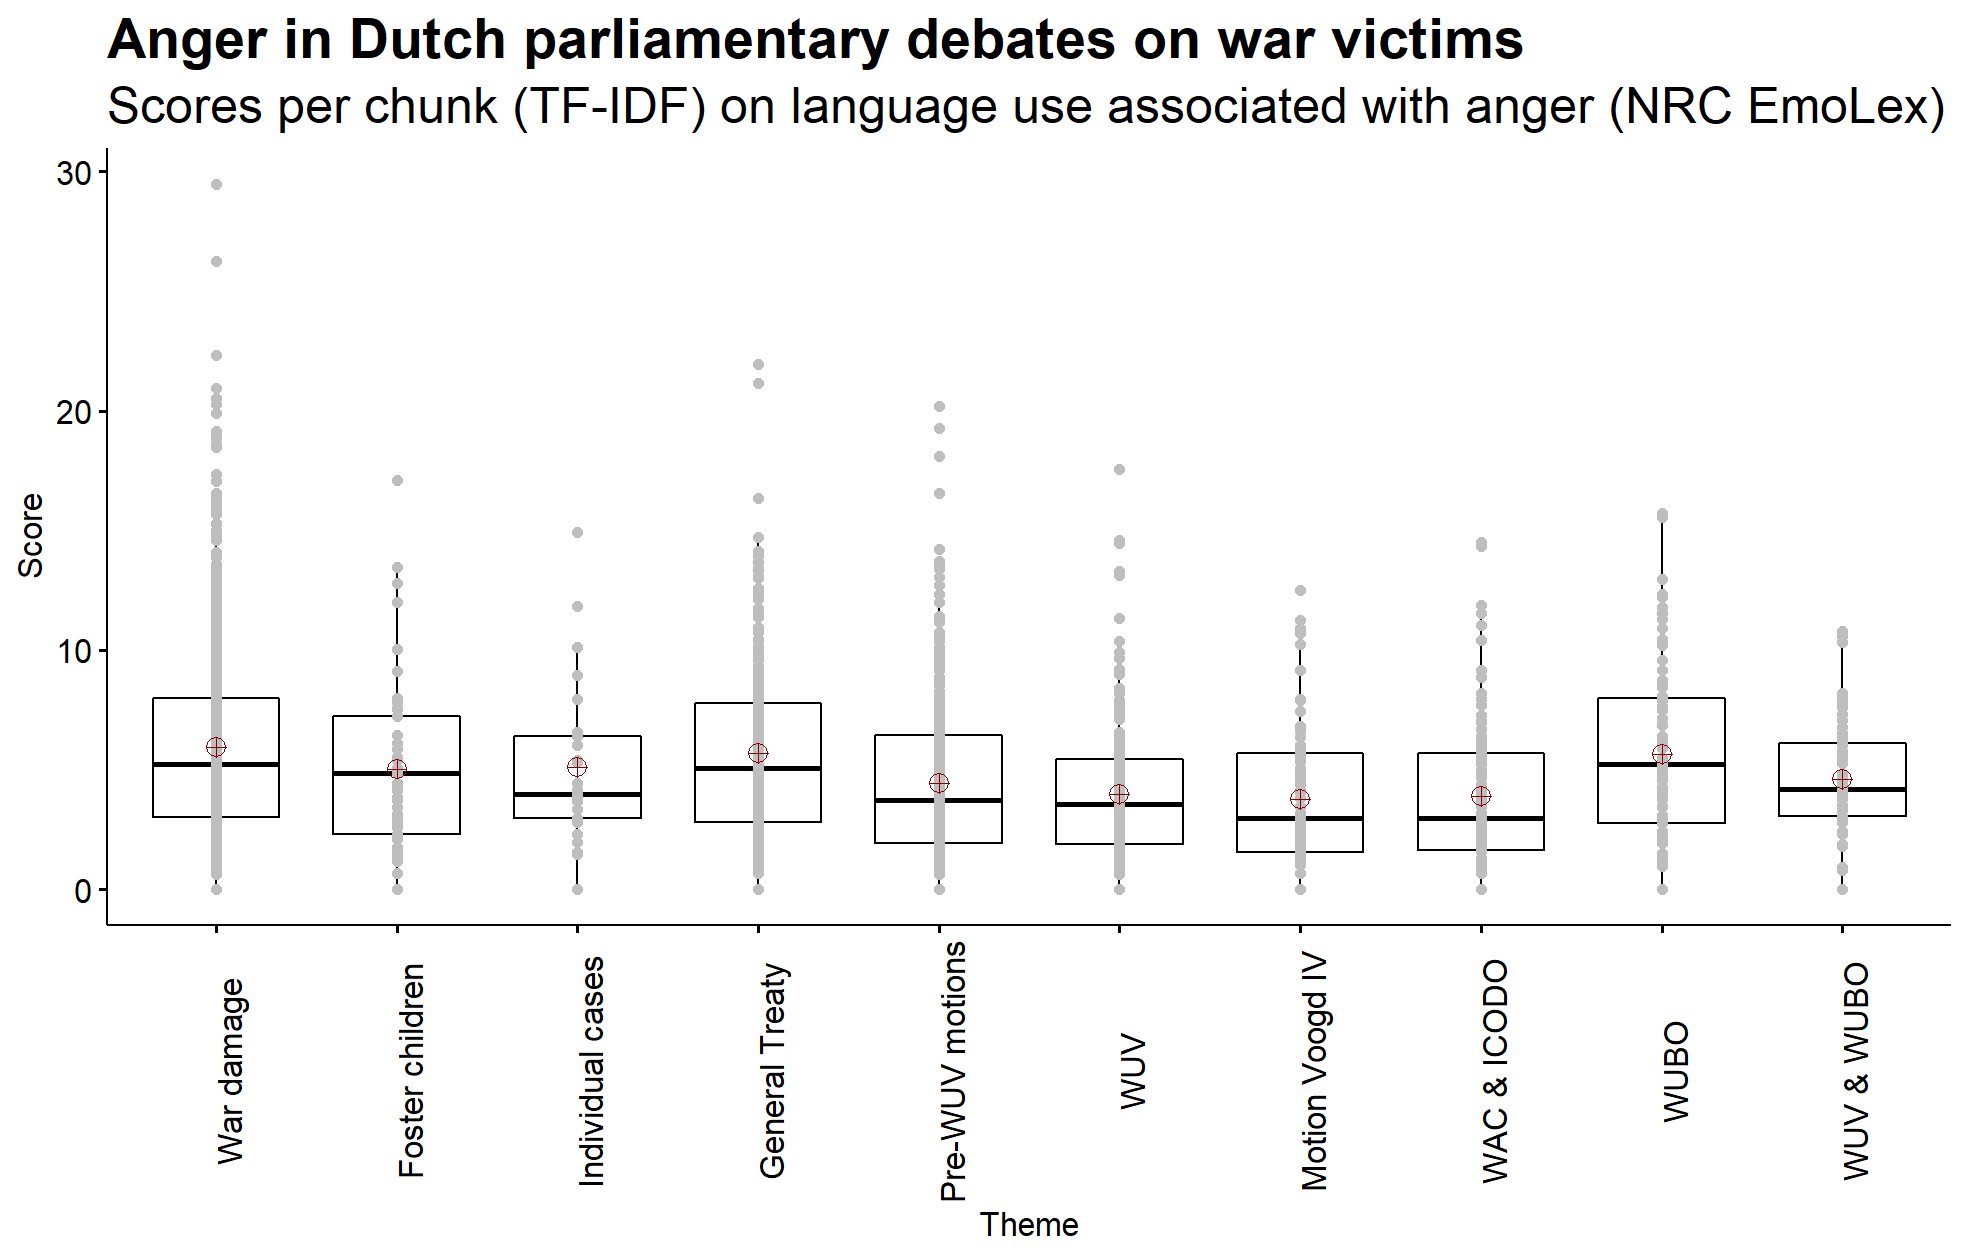
\includegraphics[width=0.9\linewidth]{Images/boxplot1.png}
    \\
    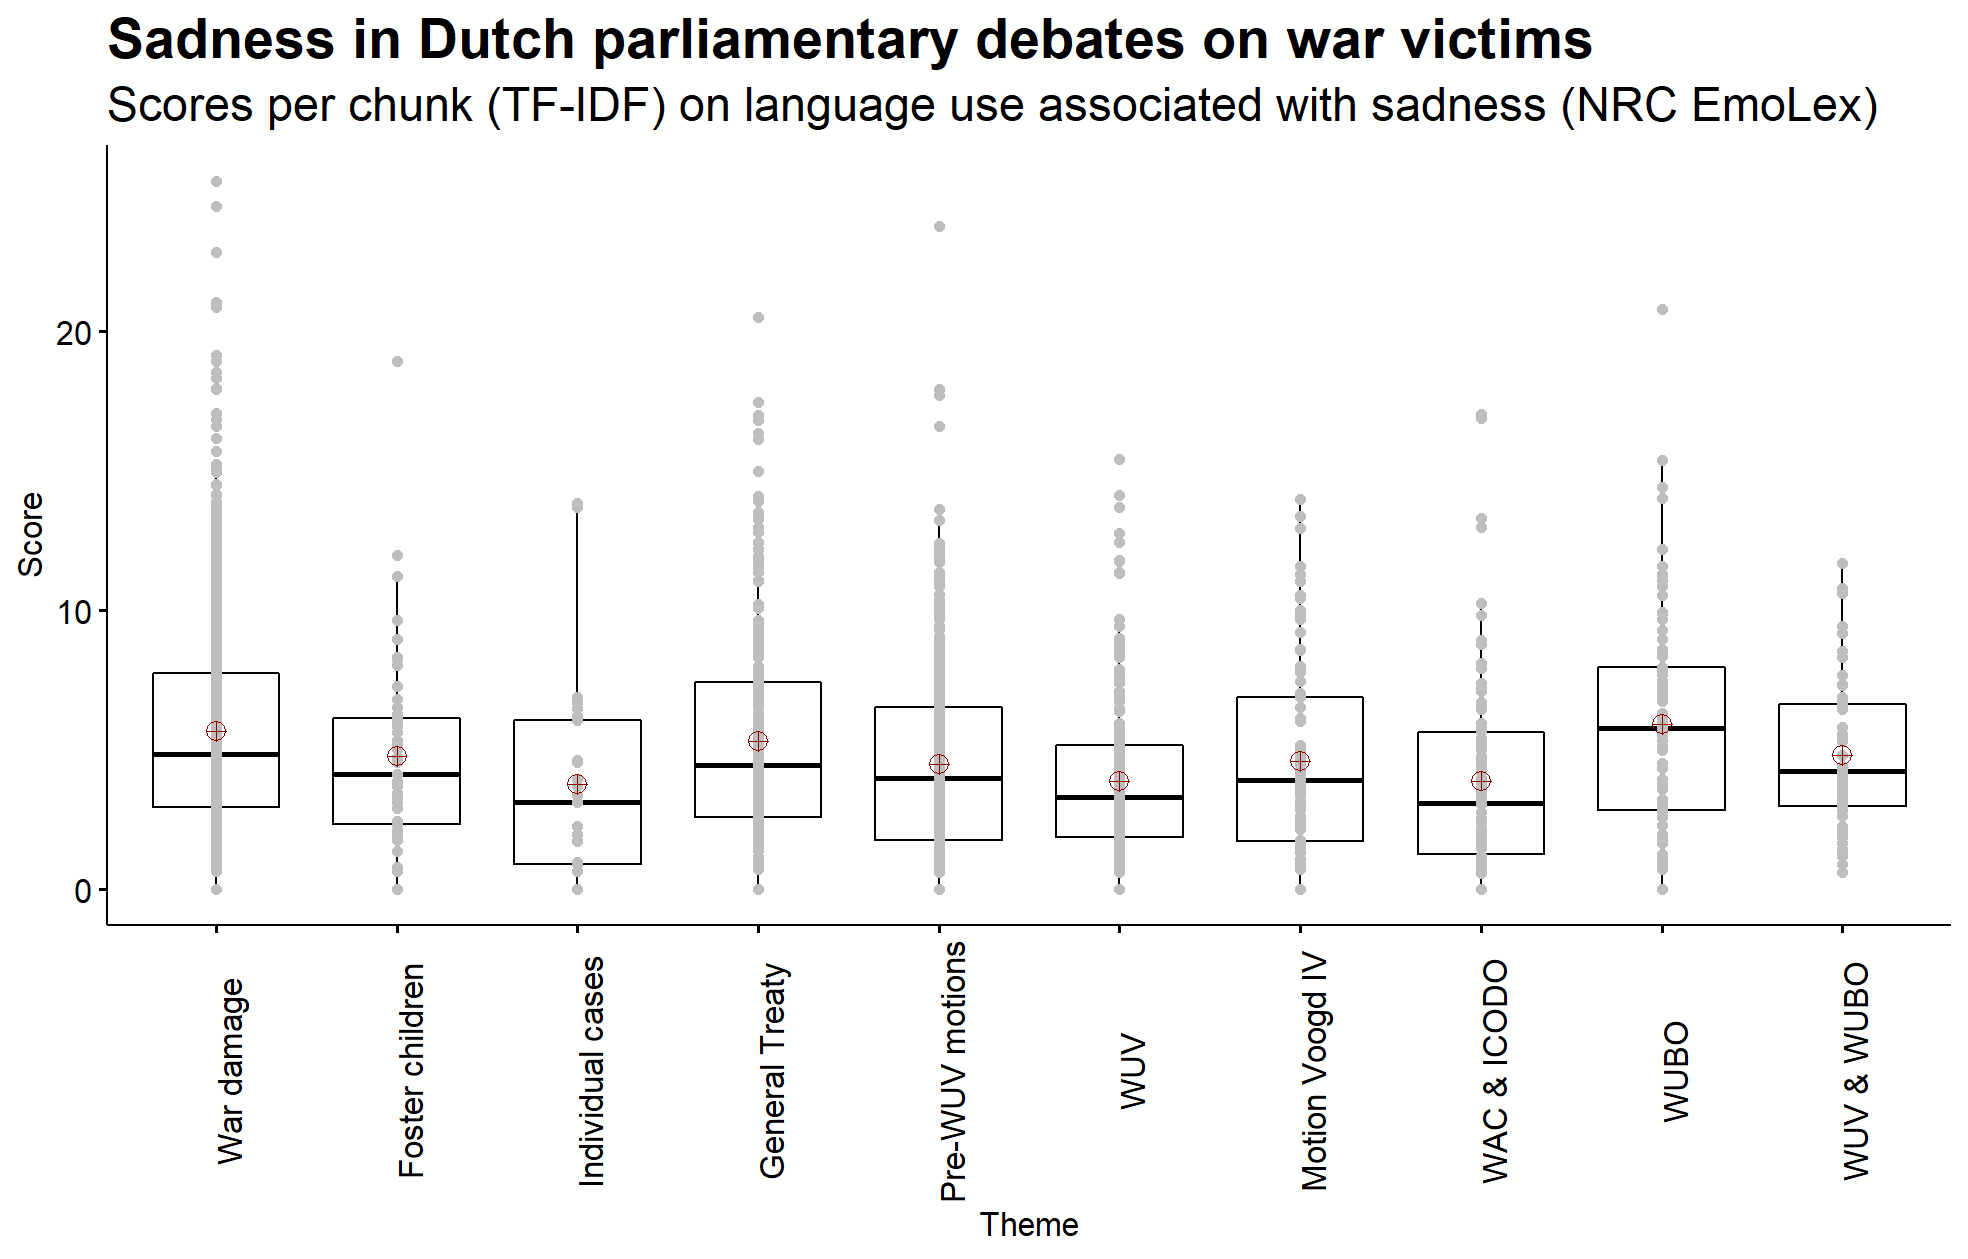
\includegraphics[width=0.9\linewidth]{Images/boxplot2.png}
    \\ 
    \end{tabular}
    \caption{Scores of each thematic cluster of war victim debates on word use associated with anger. Individual chunk scores in grey, mean in red.}
    \label{fig:boxplot}
\end{figure}

% \begin{figure}[th]
% % Use center to align a figure or table to the middle of the text column
% \begin{center}
% 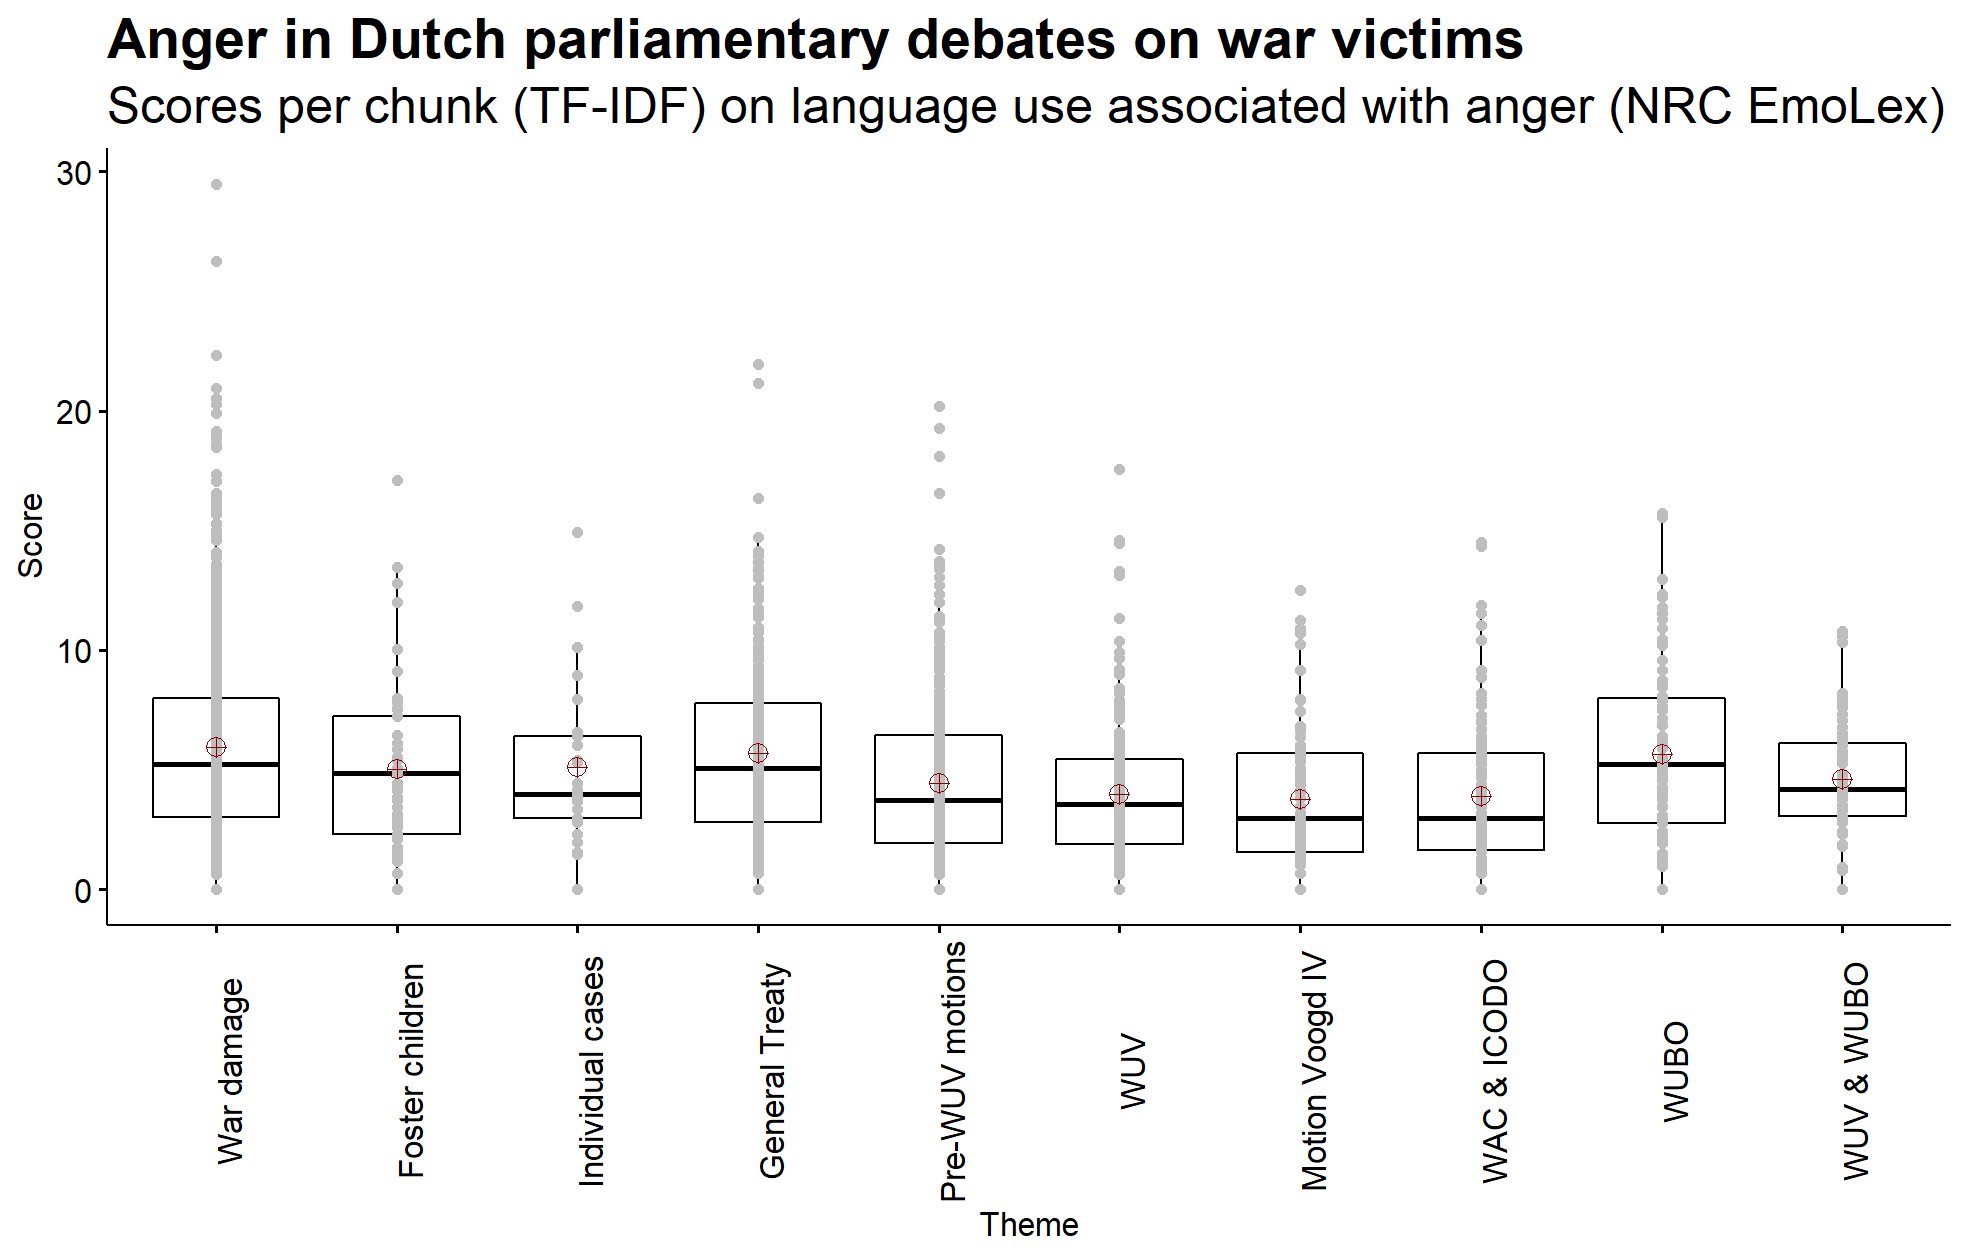
\includegraphics[width=0.9\linewidth]{Images/boxplot1.png}
% \end{center}
% \caption{Scores of each thematic cluster of war victim debates on word use associated with anger. Individual chunk scores in grey, mean in red.}
% \label{fig:boxplot1}
% \end{figure}
% %
% \begin{figure}[h]
% % Use center to align a figure or table to the middle of the text column
% \begin{center}
% 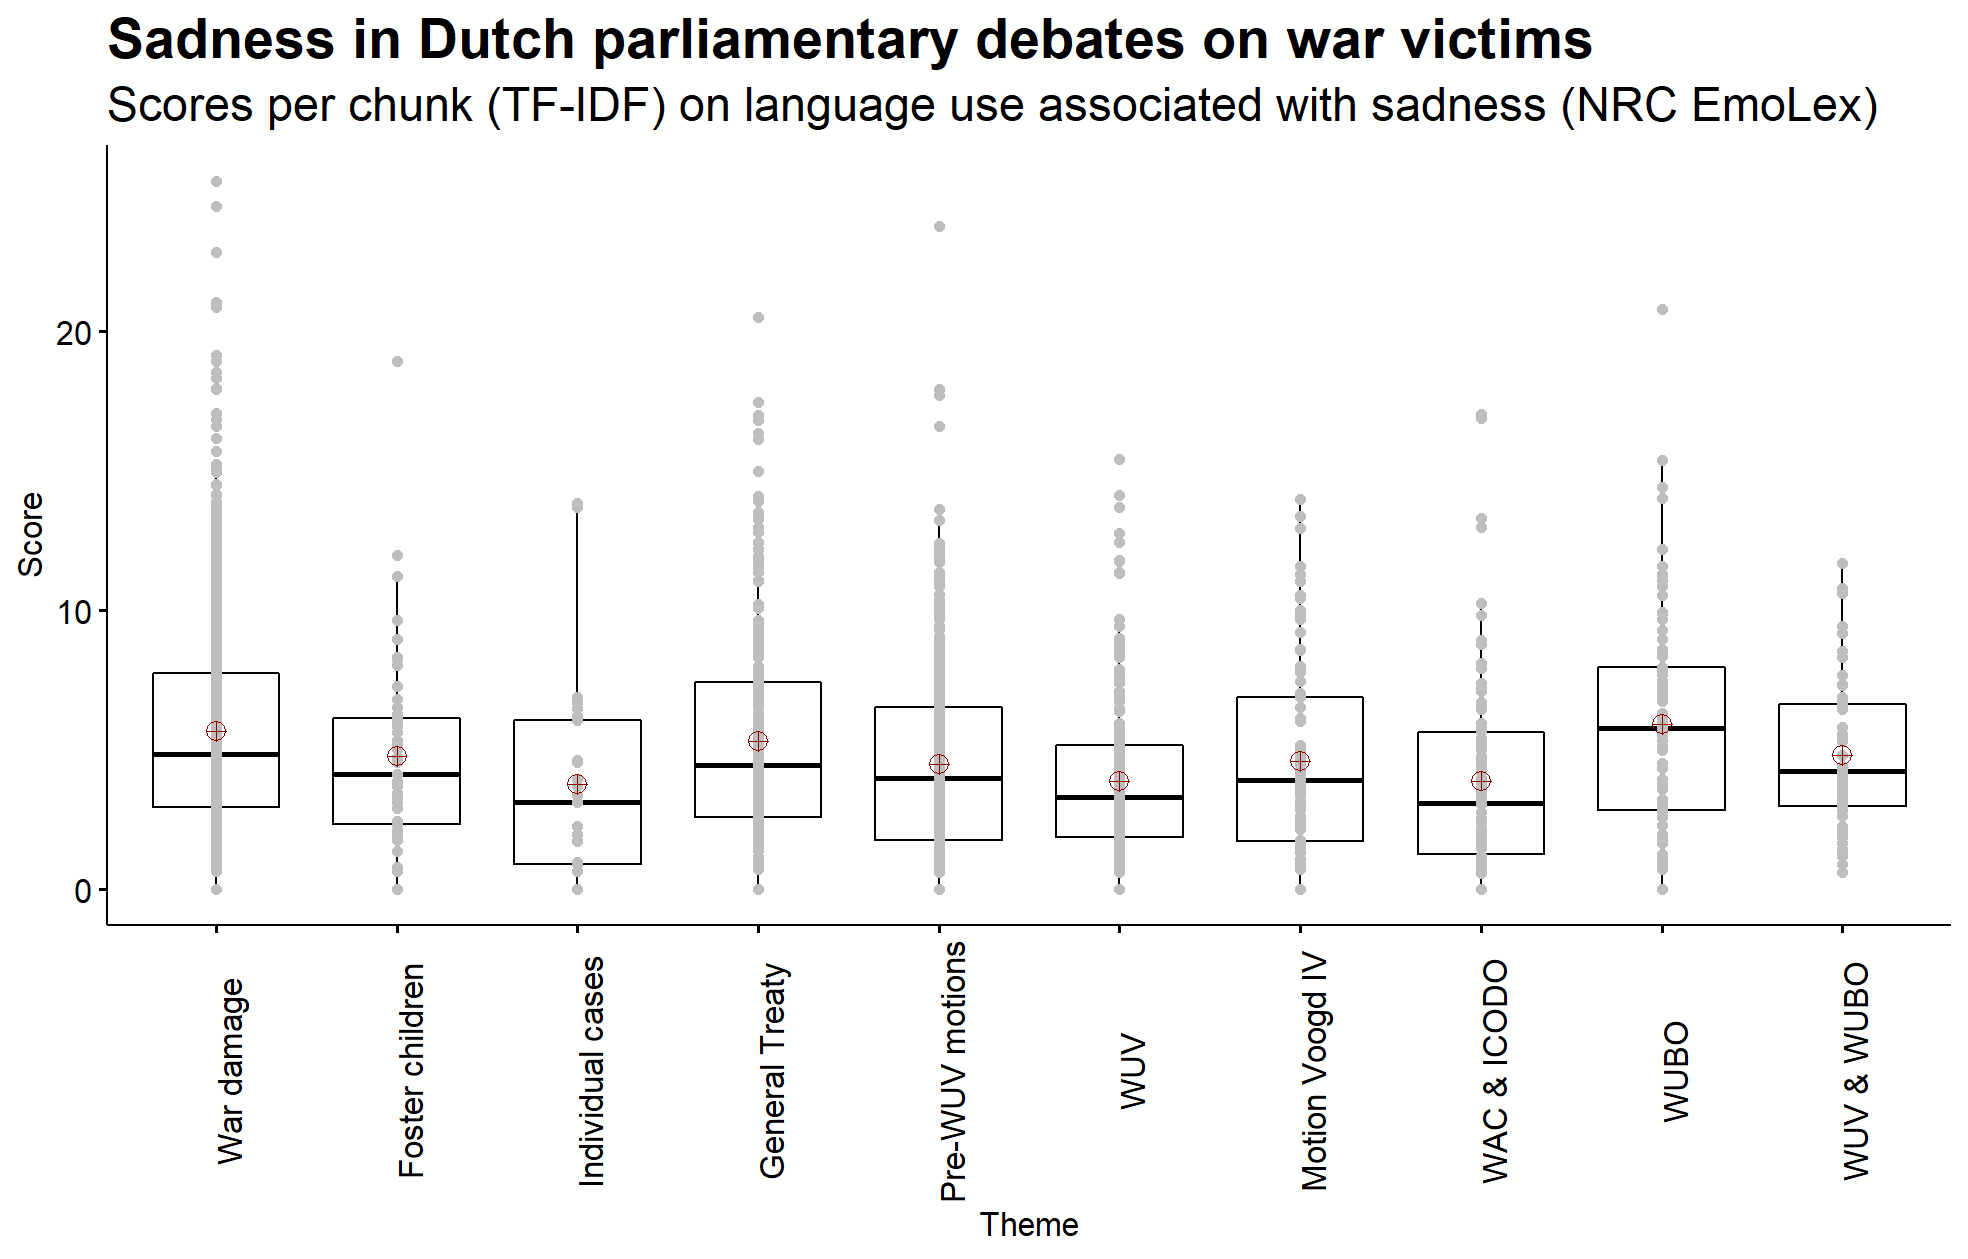
\includegraphics[width=0.9\linewidth]{Images/boxplot2.png}
% \end{center}
% \caption{Scores of each thematic cluster of war victim debates on word use associated with sadness. Individual chunk scores in grey, mean in red.}
% \label{fig:boxplot2}
% \end{figure}


\begin{figure}
    \centering
    \begin{tabular}{c}
         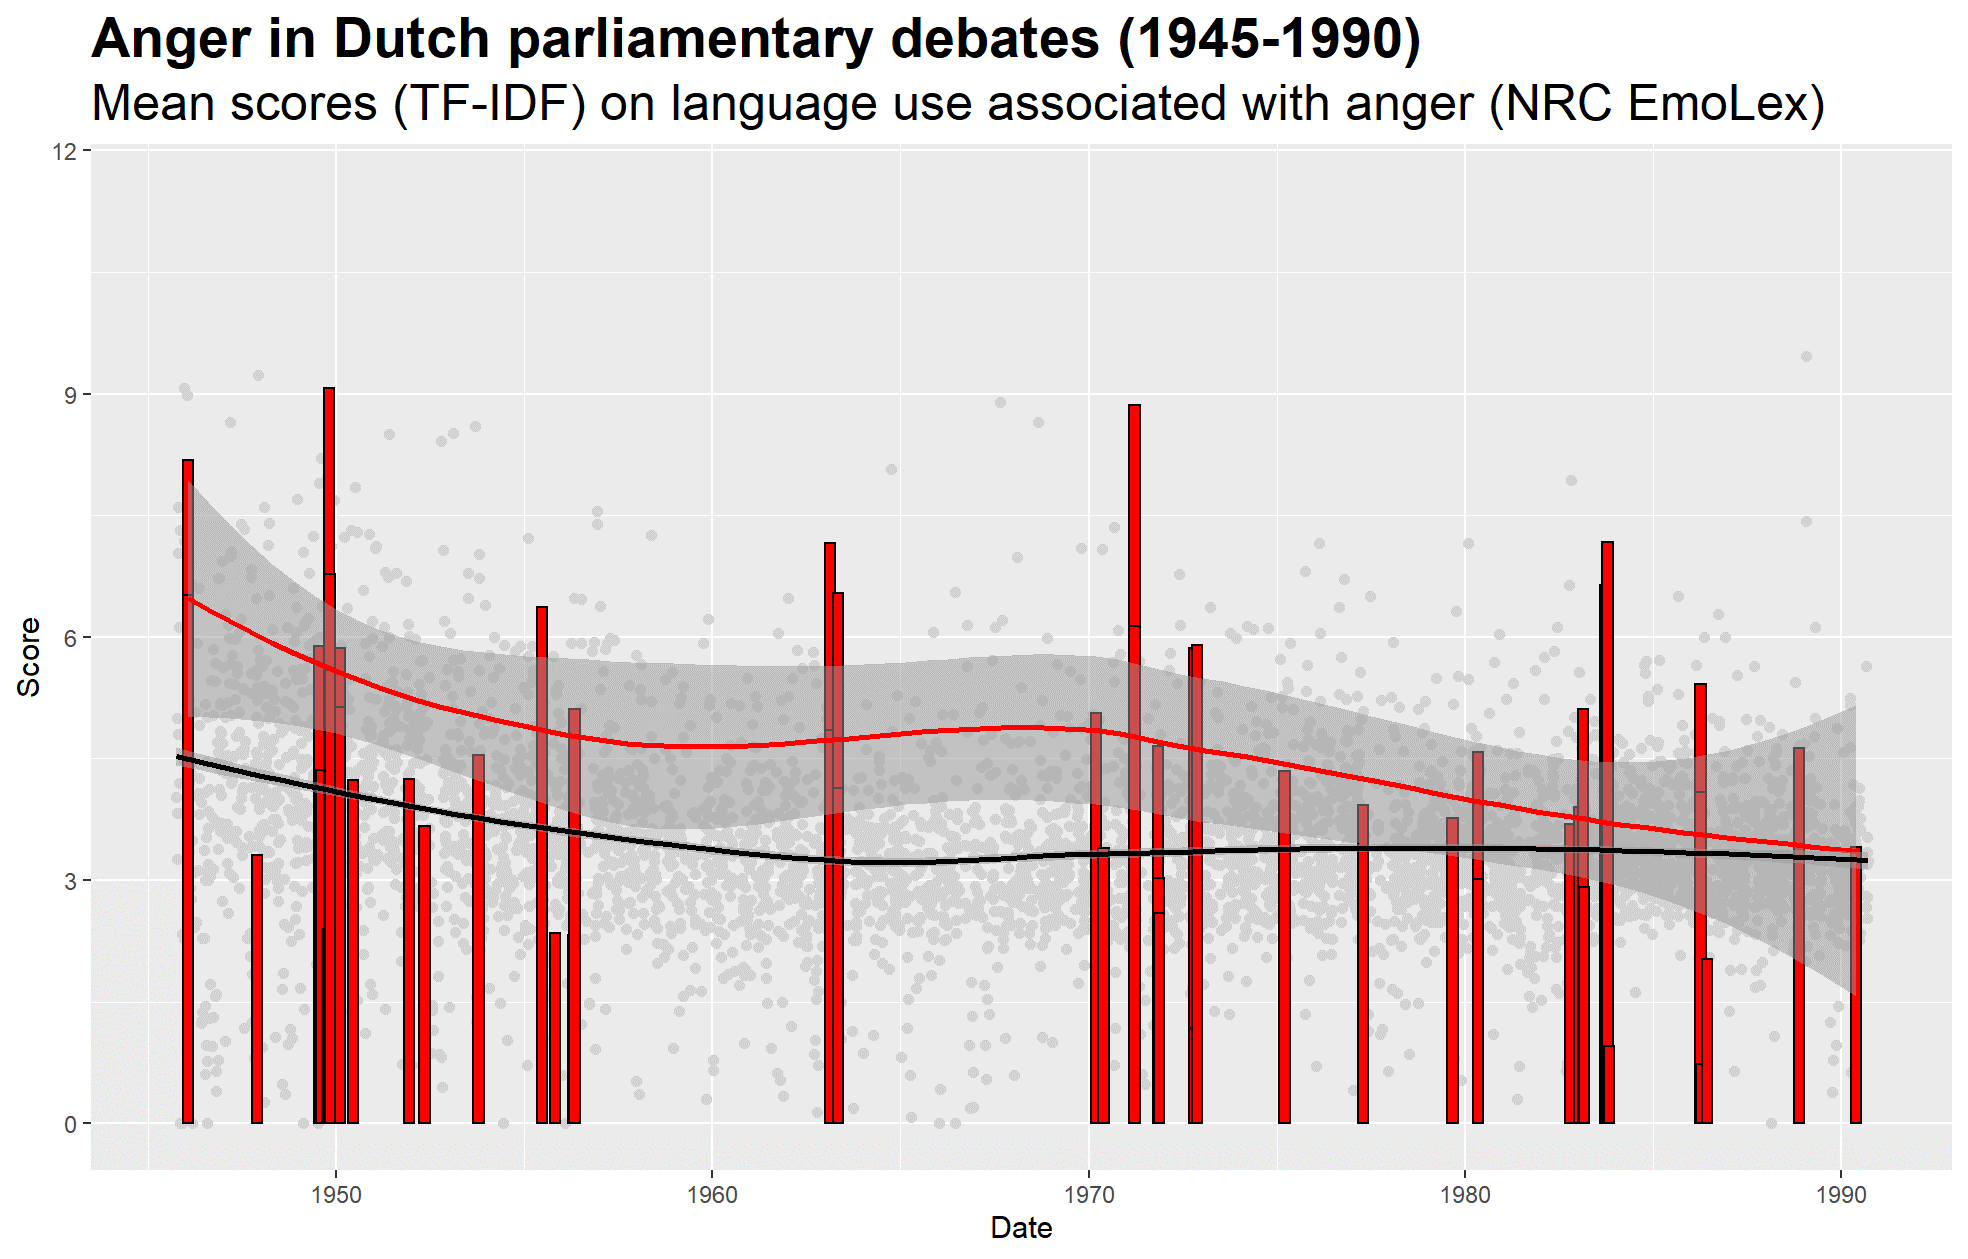
\includegraphics[width=0.9\linewidth]{Images/graph1.png} \\
         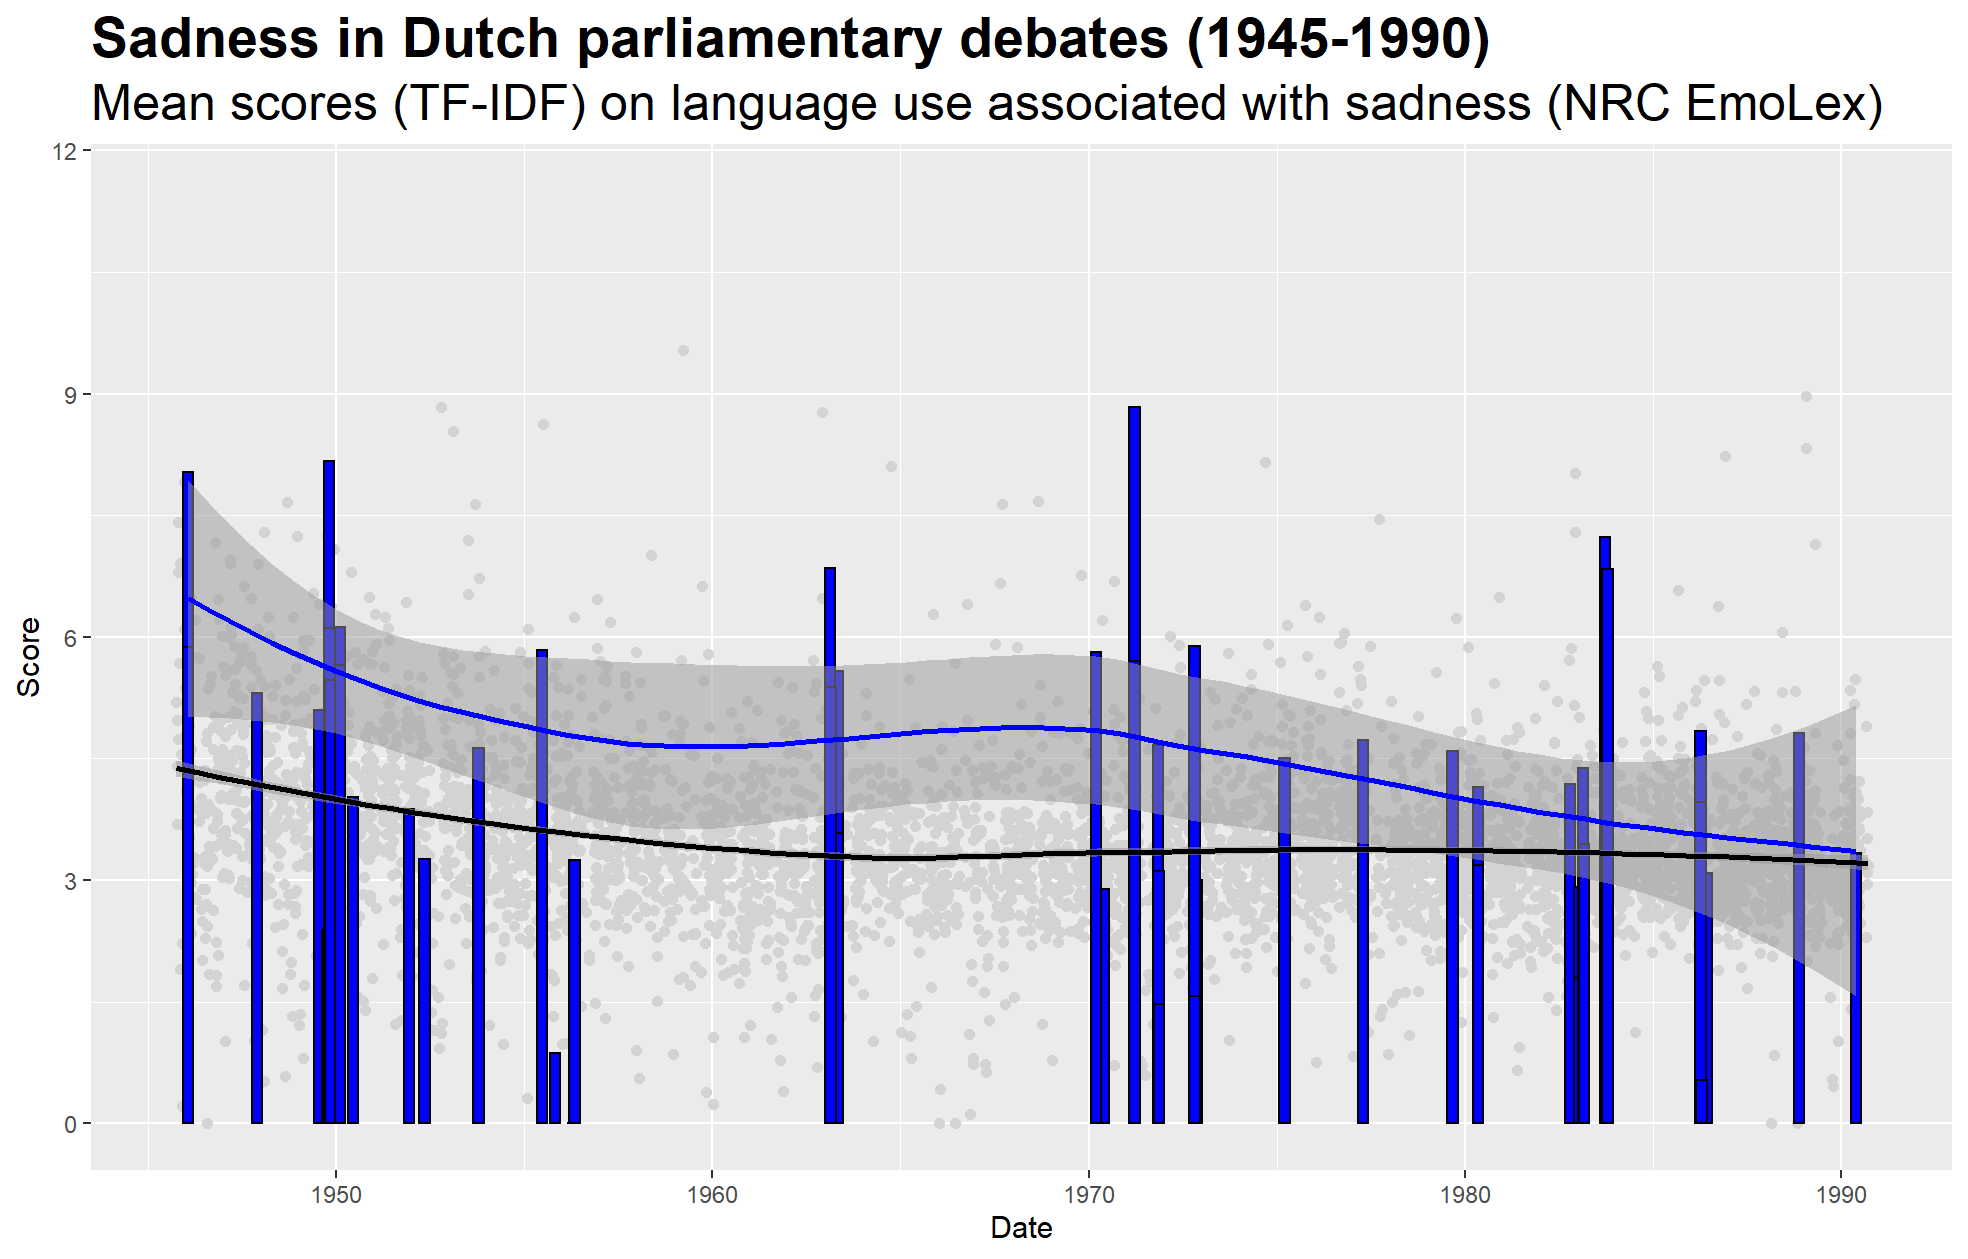
\includegraphics[width=0.9\linewidth]{Images/graph2.png} \\ 
    \end{tabular}
    \caption{Scores of each individual war victim debate and the moving average (Loess smoothing) on word use associated with the target word (in red) for `anger' at the top and for `sadness' at the bottom. All other parliamentary debates in grey (monthly mean) and black (moving average).}
    \label{fig:graph}
\end{figure}

% \begin{figure}[ht]
% % Use center to align a figure or table to the middle of the text column
% \begin{center}
% 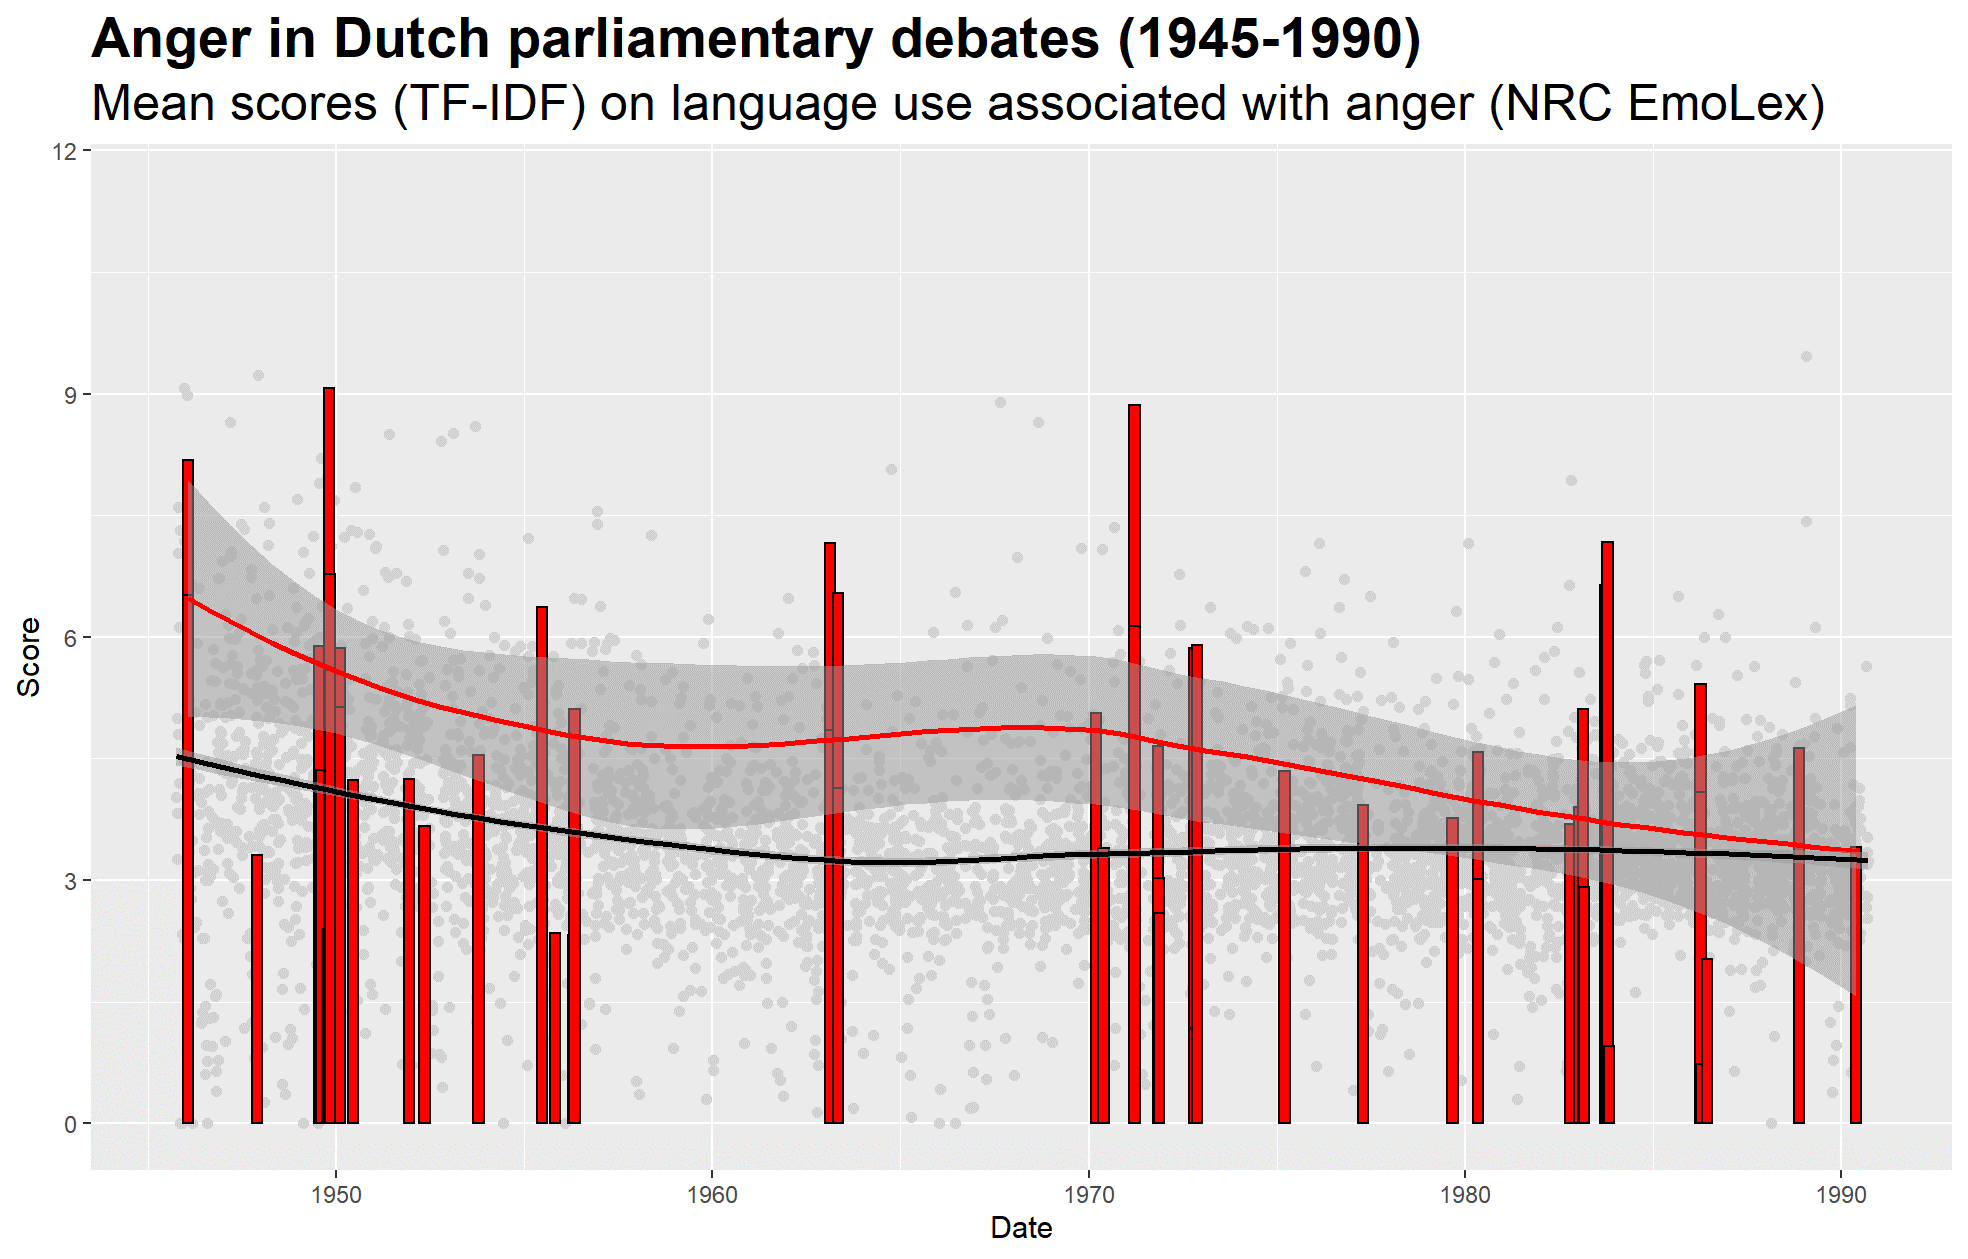
\includegraphics[width=0.9\linewidth]{Images/graph1.png}
% \end{center}
% \caption{Scores of each individual war victim debate and the moving average (Loess smoothing) on word use associated with anger (in red). All other parliamentary debates in grey (monthly mean) and black (moving average).}
% \label{fig:graph1}
% \end{figure}

% \begin{figure}[ht]
% % Use center to align a figure or table to the middle of the text column
% \begin{center}
% 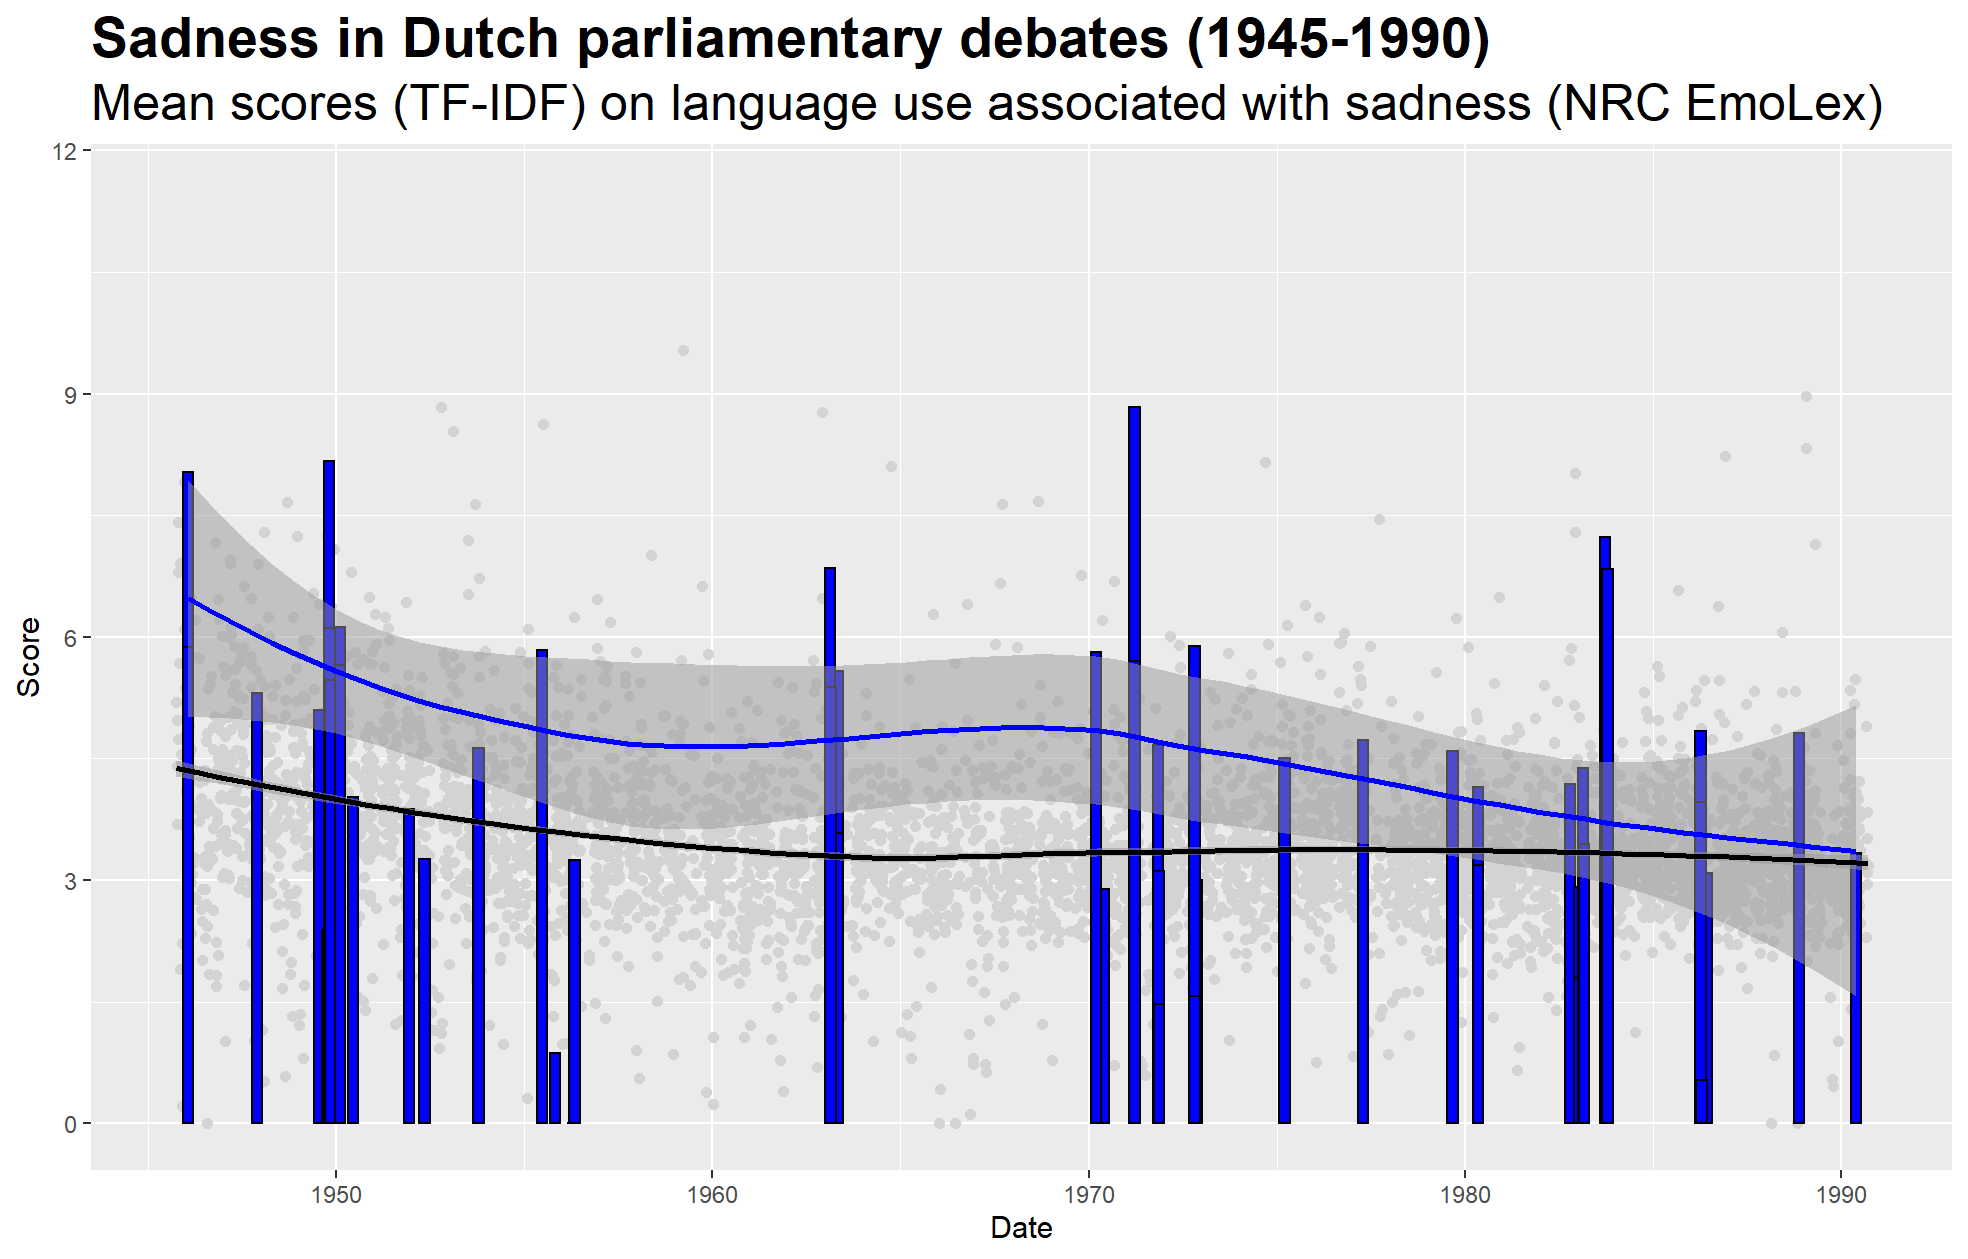
\includegraphics[width=0.9\linewidth]{Images/graph2.png}
% \end{center}
% \caption{Scores of each individual war victim debate and the moving average (Loess smoothing) on word use associated with sadness (in blue). All other parliamentary debates in grey (daily mean) and black (moving average).}
% \label{fig:graph2}
% \end{figure}

That there is little variation among the different war victim debates, is not to say we did not find any variation in emotionality in parliamentary debates at all. When we compare the war victim debates with the other parliamentary discussions, a difference in scores can be observed. Most of the debates dealing with war victim legislation score higher on the emotions anger and sadness than the average parliamentary debate. When looking at the moving average, we can say that this is true for the entire period under scrutiny.

In the timelines in 
Figure~\ref{fig:graph}, 
%Figures~\ref{fig:graph1} and~\ref{fig:graph2}, 
not only the (high) scores, but also the number of debates give no indication whatsoever of a ‘silence’ regarding this topic in Dutch parliament in the first post-war decade. The Material War Damage debates (1945-1950) in particular belong to the longest, most elaborate parliamentary discussions within the war victim debates dataset.\footnote{The MOS debates also consist of much more words than any other thematic debate cluster on other types of legislation in later years (see also Table~\ref{tab:counts}).} In addition, the high emotion scores do not indicate a withholding or suppression of language use associated with emotions in the period 1945-1960. This indicates that emotions were in this period, from a quantitative perspective, just as frequently manifest as in later debates.

When zooming in to the 'words behind the scores', the lists (see Figures~\ref{fig:top201} and~\ref{fig:top202} in section \ref{sec:app} Appendix) with the highest scoring words display a frequent use of references to emotional events (e.g. 'bombardment', 'disaster', and 'loss'), and to verbs related to suffering (e.g. 'to afflict', 'to demolish'), and suffering in general (such as 'suffer', 'grief' or 'misery').  Close reading of the actual historical debates, as a traditional historian, indicates that words as these were often used in emotional descriptions of people’s suffering. Sometimes, this was done by detailed descriptions of examples of suffering from identifiable, individual victims. These examples were used to dress up the parliamentary discussion on material war damage. Often, however, emotion words were present in generic mentions of misery. Take, for example, fragments of a speech of Pieter Zandt, member of the House of Representatives for the Reformed Political Party (SGP). He mentioned how people ``(...) have suffered (...) in the war'', and how they were ``(...) plunged in deep mourning.'' He also emphasized how people had undergone ``sorrow'' and ``misery'' \citep[p.305]{noauthor_handelingen_1949-1950}. We consider this quote exemplary for how victims' misery and related emotions were not silenced or forgotten in the 1950s. Instead, we argue, MPs frequently displayed a rather empathetic attitude. Emotional words were used extensively in rhetorical arguments for establishing elaborate and generous bills for the relief of material war damage. That is to say, of material damage. 
%
In contrast to material damage, alleviating suffering related to immaterial aspects of war victims' suffering was not seen as a governmental responsibility \citep[p.305]{noauthor_handelingen_1949-1950}. 
%Immaterial aspects of war victims' suffering was, in contrast to material damage, not considered as a government task \citep[p.305]{noauthor_handelingen_1949-1950}.

Both our 'distant' and 'close' reading results do not display a 'silence' in the 1950s – either in terms of discussing war victims, and in the manifestation of related emotions. This does not seem to be the case in the following decade (see the trend lines in 
Figure~\ref{fig:graph}). 
%Figures~\ref{fig:graph1} and~\ref{fig:graph2}). 
If there is a silence to be observed in these graphs, it consists of the period of roughly covering the 1960s – with one 1963 debate (on the General Treaty for compensation with Germany) as an exception. This lacuna in the observations, however, was more the result of an administrative policy choice or practice, than that it was related to a shift in the role of emotions in these discussions. National governmental care for war victims became integrated into the general social welfare legislation in this period. As a consequence, the decision-making processes regarding war victim-related legislation was not separately scheduled for parliamentary discussion \citep{piersma_bevochten_2010}.

Contrasting the 1950s, the alleviating of individual and consequential, late-onset suffering, also and indeed especially in immaterial terms, was considered as a governmental responsibility in the early 1970s. The emotion scores in the debates on the WUV – the first social benefit scheme particularly aimed at the contemporary and immaterial problems of war victims – are relatively similar to the scores of the debates in the 1950s. When looking at the quantitative measures, emotional manifestations still had a prominent role in discussing war victims in parliament. This does not say that nothing had changed.

A closer look at the most frequent lexicon words behind the scores, and the actual course of the debates, indicate a shift from an 'empathetic' to 'appraising' role of emotional language. Examples of emotion words used in the discussions are those directly referring to an emotion, such as 'bitterness', 'fear', or 'sadness'. Other words refer to the typical expressions of emotions, such as 'crying', a verb obviously associated with the emotion {\em sadness}. With this choice of words, MPs made explicit what kind of emotions they perceived as being present in society. In the practice of discussing the WUV, they often related them to particular groups of victims  \citep[p.101]{noauthor_handelingen_19691970-1}. Parliamentarian Norma Dettmeijer-Labberton (Liberal Party, VVD), for example, explicitely emphasized that the emotions of especially Jewish victims of Nazi persecution had to be addressed in the development of future legislative schemes  \citep[p.3473–74, 3490–91]{noauthor_handelingen_1970-1971-2}. 

To summarize the observed development more concretely: emotional language use in the 1970s discussions changed from using 'words associated with certain emotions' to 'words explicitly referring to a certain emotion'. Instead of describing victims' misery in an evocative manner, as was done in the 1950s by outlining 'losses' and 'disasters' in adjective-laden diatribes, MPs' appraisals of related sadness, bitterness, or fear (of others) dominated in the debates of the 1970s. In other words, in the 1950s politicians spoke emotionally, whereas in the 1970s they spoke about emotions. This is backed up in particular by the most frequently used words related to sadness. Examples of frequently occurring words explicitly referring to emotions are: 'fear', 'regret', 'bitter', 'bitterness', or 'sorrow'. Other words refer to the typical expressions of emotions, such as aforementioned example of the verb 'crying'. This qualitative change, however, was not yet indicated by the quantitative emotion mining results, as no significant linear increase in the use of anger and sadness words between 1945 and 1990 has been found. This is where the top word lists of emotion lexicon words proved particularly insightful (see also the tables in section \ref{sec:app} Appendix).

\section{Conclusion} 
In this paper, parliamentary debates were analysed to investigate a persistent periodization in Dutch historiography of the post-war dealing with the immediate and late consequences of World War II in the Netherlands. We wanted to know whether this periodization (or cycle), in which emotions seem to play a key role, could be discerned in parliamentary language use by analysing parliamentary proceedings with an external perspective of lexicon-based emotion mining.

Results of emotion mining in this investigation helped indicate, in the first place, outliers (or the lack thereof), and assisted in describing diachronic trends on a very rough level. A first important finding is that most – not all – debates on war victim legislation score higher on word use associated with anger and sadness than the average parliamentary debate. This is true for the entire period we have investigated (1945-1990). The quantitative results pointed at the elaborate and relative emotional discussions of the late 1940s and 1950s on the Material War Damage Act (MOS). 

How do the outcomes of this investigation compare to the common view of emotionality in this period as presented by various historians? Withuis, Beunders, Aerts and others have emphasised clearly observable periods of heightened and subdued emotionality. Emotion mining outputs, by contrast, indicated first and foremost a relatively stable trend in manifestations of emotional language - especially in the average, non-war victim-related parliamentary debates. When looking at the war victim debates in particular, a relative peak in emotion scores was observed in the first post-war years, including the early 1950s. Subsequently, the diachronic emotion mining output displayed a minor decreasing trend in the war victim debates. Aside from a very minor revival in the scores around 1970, the decreasing trend that started after 1945 continued until the end of the 1980s. 

This investigation has found no empirical evidence of a 'silencing' in parliament regarding the suffering of war victims, or regarding related emotions, in the first 15 years after the allied liberation of 1945. There was, in the first place, elaborate discussion. Victims were discussed in parliament in the context of the Material War Damage Act. Secondly, as a closer scrutiny of debates indicated, emotional descriptions of suffering of identifiable war victims were used to dress up arguments for elaborate and generous legislation or compensation. Our analysis indicated that contemporary MPs did not have a 'stiff upper lip', as the elaborate attention for individual suffering – expressed in particularly emotional language – displayed first and foremost an empathetic attitude. That the resulting legislation of the 1950s was considered as rather limited in hindsight, did not mean contemporary parliamentarians had no eye for personal war-related suffering. Neither, moreover, did we find empirical evidence for a strong quantitative increase in emotionality in later decades. We argue that the term 'emancipation' that is used in historiography to refer to the developments in the 1970s is somewhat confusing, as it implies that there had been close to no space for the manifestation and expression of emotions before.\footnote{Why and how this presumption of 'silence' that was followed by a process of 'emancipation' became so prominent, both in contemporary debates as in the later historiography, will be further examined in a chapter of the dissertation \textit{Emotional Imprints} that builds on this research.}

If there is a conclusion to be drawn regarding 'silence' in the emotion mining results, it is a lacuna in the emotion scores of the 1960s. The lack of substantial parliamentary debate in those years, however, had more to do with contemporary administrative and organizational practices, than with silencing or withholding emotions. As war victim legislation was not discussed separately, it was difficult to confront close reading of these debates with a distant reading perspective. This is an unfortunate, but inevitable limitation of this type of research material and our quantitative approach – as the latter requires a rather rigid categorization of debates.

That emotional manifestations were a relative constant in parliamentary debates over more than four decades, does not mean that nothing had changed. We would argue that utilising more traditional historical research practices alongside emotion mining proved valuable. Closer scrutiny of the words behind the scores, and the actual debates, was necessary to gain more detailed insight in what was actually going on. Closer scrutiny of the most frequent lexicon words behind the scores indicated a shift in language from using 'words associated with certain emotions' to 'words used to explicitly refer to a certain emotion'. Emotion mining output had an indicative function in this investigation, but did not draw a comprehensive picture of developments, changes, or how above-mentioned 'qualitative change' unfolded in the debates. Closer scrutiny of the lexicon words behind the scores and close reading of the original documents remained essential to understand, interpret, and give meaning to the details of complex and multifaceted historical developments, continuities, and changes.

Were the previous historians writing on this topic (all) wrong? Perhaps. As we explained, the computational methods and resources used here are not without limitations. On the other hand, it is difficult if not impossible to grow up Dutch without developing strong ideas about World War II and its aftermath. We think it is more likely, although not certain, that our emotion mining results have helped identifying a shared preconception in historiography, rather than a shortcoming of lexicon-driven emotion mining.

\bibliography{references}

\newpage
\section{Appendix}
\label{sec:app}
All other data, graphs, and table used in/referred to in this paper can be found in: Data Repository ‘Vehemence and Victims’ (version 1). Amsterdam: NIOD, 2020. https://github.com/MilanvanL/vehemence-victims.


\begin{figure}[h]
\begin{center}
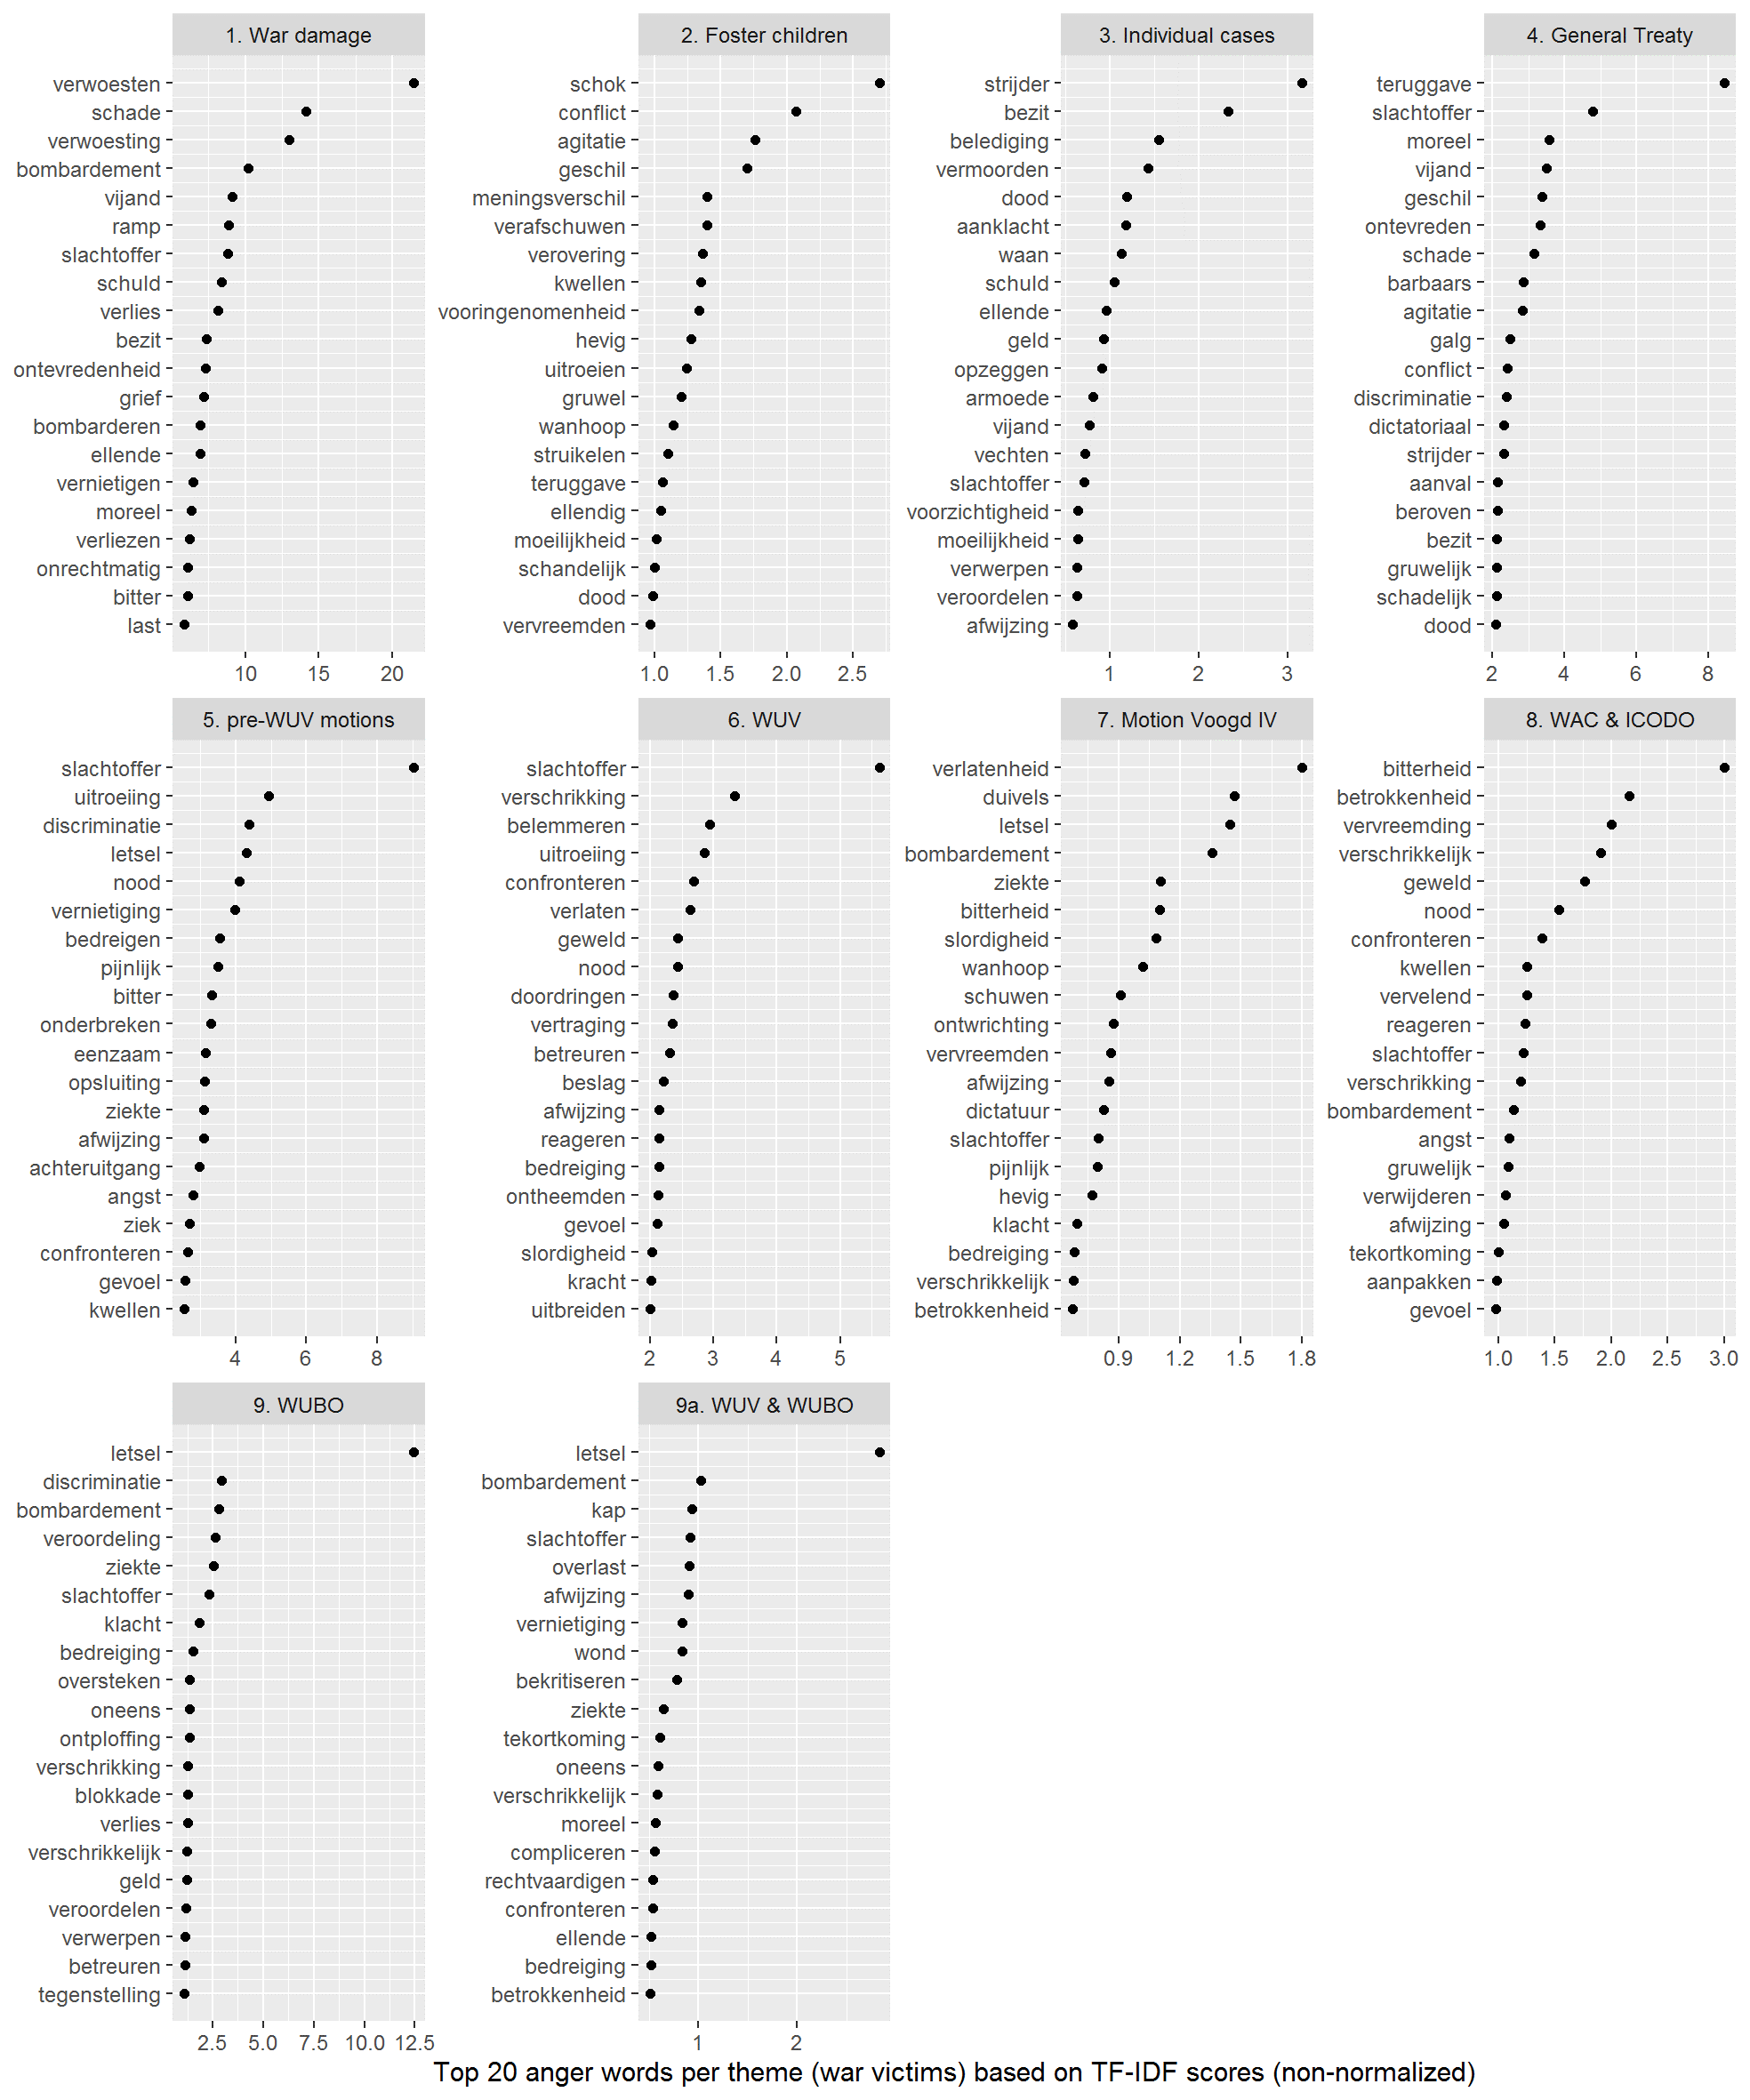
\includegraphics[width=0.8\linewidth]{Images/top201.png}
\end{center}
\caption{Top 20 (Dutch) anger words (NRC EmoLex) per thematic cluster of war victim-related parliamentary debate}
\label{fig:top201}
\end{figure}

\begin{figure}
\begin{center}
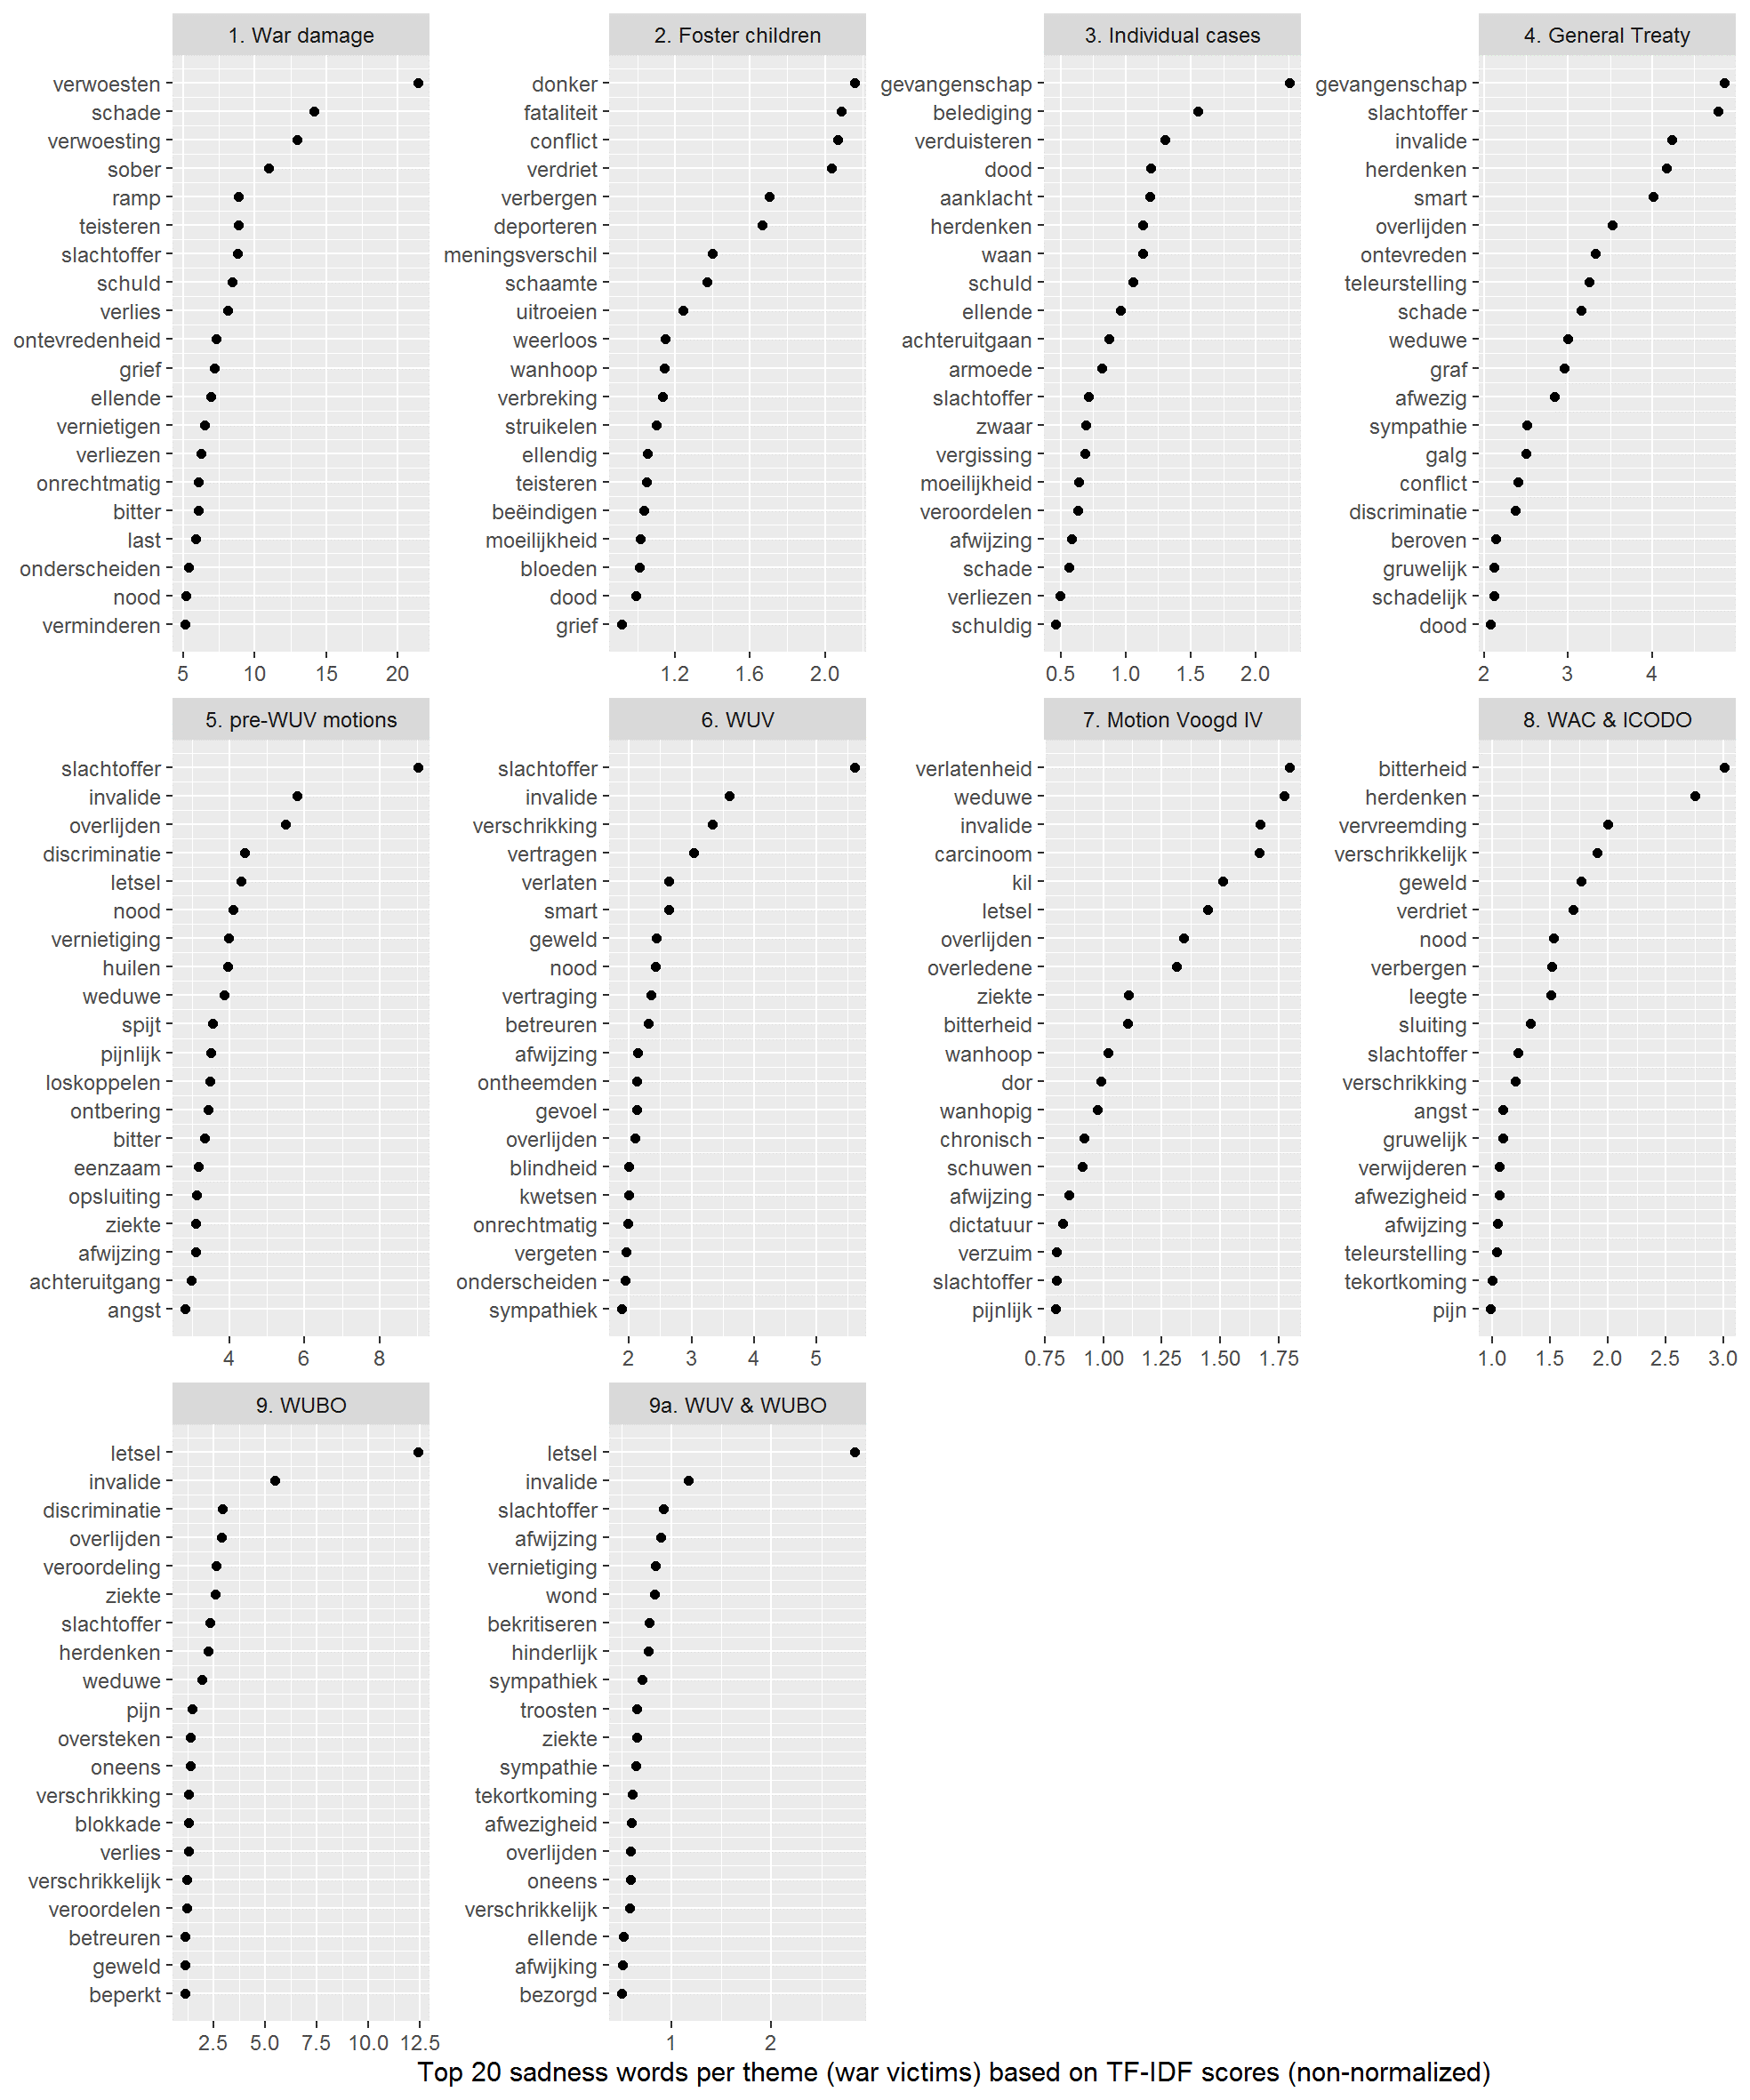
\includegraphics[width=0.8\linewidth]{Images/top202.png}
\end{center}
\caption{Top 20 (Dutch) sadness words (NRC EmoLex) per thematic cluster of war victim-related parliamentary debate}
\label{fig:top202}
\end{figure}
\end{document}
